\documentclass[12pt,spanish,openany,letterpaper,pagesize]{scrbook}
\usepackage[utf8]{inputenc}
\usepackage[spanish]{babel}%escribir con acentos sin necesidad de comandos \'{} .
\usepackage{fancyhdr}
%\usepackage{epsfig}
\usepackage{epic}
\usepackage{eepic}
\usepackage{amsmath, amssymb, amsthm, latexsym, graphics, graphpap, layout, wasysym, multicol, enumerate,amsfonts,mathrsfs}
\usepackage{graphics,lscape}
\usepackage[mathscr]{euscript}
\usepackage{xcolor}
\usepackage{verbatim}
\usepackage{booktabs}
\usepackage{float}
%\usepackage{hyperref}
\usepackage{threeparttable}
\usepackage{amscd}
\usepackage{here}
\usepackage[pdftex]{graphicx}
\usepackage{lscape}
\usepackage{tabularx}
\usepackage{subfigure}
\usepackage{longtable}
\usepackage{geometry}
\usepackage{cite}
\usepackage{algorithmic}
\usepackage{diagbox}
\usepackage{array,multirow}
\usepackage[all]{ xy}
\usepackage[hidelinks]{hyperref}

\usepackage{graphicx}
\usepackage{caption}
\usepackage{subcaption}
\usepackage{subfig}

\usepackage{rotating} %Para rotar texto, objetos y tablas seite. No se ve en DVI solo en PS. Seite 328 Hundebuch
                        %se usa junto con \rotate, \sidewidestable ....
                        

\renewcommand{\theequation}{\thechapter-\arabic{equation}}
\renewcommand{\thefigure}{\textbf{\thechapter-\arabic{figure}}}
\renewcommand{\thetable}{\textbf{\thechapter-\arabic{table}}}

\pagestyle{fancyplain}%\addtolength{\headwidth}{\marginparwidth}
\textheight22.5cm \topmargin0cm \textwidth16.5cm
\oddsidemargin0.5cm \evensidemargin-0.5cm%
\renewcommand{\chaptermark}[1]{\markboth{\thechapter\; #1}{}}
\renewcommand{\sectionmark}[1]{\markright{\thesection\; #1}}
\lhead[\fancyplain{}{\thepage}]{\fancyplain{}{\rightmark}}
\rhead[\fancyplain{}{\leftmark}]{\fancyplain{}{\thepage}}
\fancyfoot{}
\thispagestyle{fancy}%

\addtolength{\headwidth}{0cm}
\unitlength1mm %Define la unidad LE para Figuras
%\mathindent0cm %Define la distancia de las formulas al texto,  fleqn las %descentra
\marginparwidth0cm
\parindent0cm %Define la distancia de la primera linea de un parrafo a la margen

%Para tablas,  redefine el backslash en tablas donde se define la posici\'{o}n del texto en las
%casillas (con \centering \raggedright o \raggedleft)
\newcommand{\PreserveBackslash}[1]{\let\temp=\\#1\let\\=\temp}
\let\PBS=\PreserveBackslash

%Espacio entre lineas
\renewcommand{\baselinestretch}{1.1}

%Neuer Befehl f\"{u}r die Tabelle Eigenschaften der Aktivkohlen
\newcommand{\arr}[1]{\raisebox{1.5ex}[0cm][0cm]{#1}}

%Neue Kommandos
\usepackage{Befehle}
%Inicio del documento. Tener en cuenta que hay archivos auxiliares

\newtheorem{teor}{Teorema}[section]
\theoremstyle{definition}
\newtheorem{definition}[teor]{Definición}
\newtheorem{teorema}[teor]{Teorema}
%\newtheorem{defi}{{\textbf{Definición}}}[chapter]
%\theoremstyle{example}
\newtheorem{example}[teor]{Ejemplo}
\newtheorem{lema}[teor]{Lema}
\newtheorem{afirmacion}[teor]{Afirmación}
\newtheorem{proposicion}[teor]{Proposición}
\newtheorem{coro}[teor]{Corolario}
\newtheorem{ole}[teor]{Conjetura}

%\theoremstyle{proposicion}

%\def\proof{\paragraph{Demostración:\\}}%\begin{proof}
%\def\endproof{\hfill$\blacksquare$}%\end{proof}

\begin{document}
\pagenumbering{roman}
%\newpage
%\setcounter{page}{1}
\begin{center}
\begin{figure}
\centering%

\includegraphics[scale=0.4]{Imagenes/logo_1.png}
%{file=uc.jpg,scale=1}%
\end{figure}
\thispagestyle{empty} \vspace*{2.0cm} \textbf{\huge
Predicción del comportamiento de una enfermedad simulada en autómatas celulares con un algoritmo propuesto en redes neuronales}\\[6.0cm]
\Large\textbf{Jorge Andrés Ibáñez Huertas}\\[4.0cm]
\small Universidad Central\\
Departamento de Matemáticas\\
Bogotá, Colombia\\
2021\\
\end{center}

\newpage{\pagestyle{empty}\cleardoublepage}

\newpage
\begin{center}
\thispagestyle{empty} \vspace*{0cm} \textbf{\huge
Predicción del comportamiento de una enfermedad simulada en autómatas celulares con un algoritmo propuesto en redes neuronales}\\[3.5cm]
\Large\textbf{Jorge Andrés Ibáñez Huertas}\\[3.0cm]
\small Trabajo de grado presentado como requisito parcial para optar al
t\'{\i}tulo de:\\
\textbf{Matemático}\\[3.0cm]
Director:\\
Carlos Isaac Zainea\\[3.5cm]
Universidad Central\\
Departamento de Matemáticas\\
Bogotá, Colombia\\
2021\\
\end{center}

\newpage{\pagestyle{empty}\cleardoublepage}

% \newpage
% \thispagestyle{empty} \textbf{}\normalsize
% \\\\\\%
% \textit{"Tan sólo por la educación puede el hombre llegar a ser hombre.\\ El hombre no es más que lo que la educación hace de él"\\
% \textit{Immanuel Kant}}\\[4.0cm]

\begin{flushright}
\begin{minipage}{8cm}
    \noindent
        \small
\end{minipage}
\end{flushright}

\newpage{\pagestyle{empty}\cleardoublepage}

\newpage
\thispagestyle{empty} \textbf{}\normalsize
\\\\\\%
\textbf{\LARGE Agradecimientos}\\

El trabajo realizado en la presente tesis no habría comenzado sin la guía y los consejos de mi tutor Isaac Zainea y del profesor Nicolas Avilán. A ellos les doy mi más sincero agradecimiento por escuchar mis ideas y ayudarme a materializarlas. Por haberme introducido en las ciencias de la computación, el modelado y la simulación de eventos reales. \\

Quiero agradecer también a los profesores del departamento de matemáticas, en particular al profesor Henry Sánchez por sus consejos durante el desarrollo de esta tesis. Asimismo estoy muy agradecido con las profesoras Diana Pulido, Xiomara Rojas y Diana Herrera por sus consejos en mis años de estudio. Agradezco también a la profesora Edel Maria Serrano Iglesias (Q.E.P.D), ya que sin ella no hubiera entrado al mundo de las matemáticas. \\

Por último, agradezco a mi familia, en particular a mis padres Alexandra Huertas y Jorge Ibáñez que siempre han estado a mi lado de manera incondicional. Fue gracias a su apoyo y sacrificio que pude llegar tan lejos.

\newpage{\pagestyle{empty}\cleardoublepage}

\newpage
\textbf{\LARGE Resumen}\\

% En este trabajo se desarrollan los resultados obtenidos en el artículo  de Morales \& Arbieto,  específicamente la distancia $GH^0$ dada en ese manuscrito. Una vez se haya comprendido la fundamentación y  analizado algunas propiedades de dicha métrica, se procederá a estudiar la estabilidad topológica de las dinámicas sobre espacios compactos utilizando en principio la noción de Walters con una métrica $C^0$. Luego, se define y analiza la noción de $GH$-estabilidad  resaltando la relación que existe entre ambas nociones.\\

\textbf{\LARGE Abstract}\\\\

% In this work the results obtained in the article by Morales \& Arbieto are developed, specifically, the distance $ GH^0$ given in the article. Once the foundation is understood and some properties of that metric have been analyzed, we will proceed to study the topological stability of the dynamics on compact spaces using a notion given by Walters with a  $C^0$-metric. After that, will be defined and analyzed the $GH$-stability notion highlighting the relationship between both notions.

\renewcommand{\tablename}{\textbf{Tabla}}
\renewcommand{\figurename}{\textbf{Figura}}
\renewcommand{\listtablename}{Lista de Tablas}
\renewcommand{\listfigurename}{Lista de Figuras}
\renewcommand{\contentsname}{Contenido}

%\newcommand{\clearemptydoublepage}{\newpage{\pagestyle{empty}\cleardoublepage}}
\cleardoublepage
\addcontentsline{toc}{chapter}{Lista de figuras} % para que aparezca en el indice de contenidos
\listoffigures % indice de figuras

%\cleardoublepage
\addcontentsline{toc}{chapter}{Lista de tablas} % para que aparezca en el indice de contenidos
\listoftables % indice de tablas

\tableofcontents %% this produces the table of contents - you might have guessed :-)

%\include{Tab_Simbolos/TabSimbolosMSc}
%\include{Resumen}%\newcommand{\clearemptydoublepage}{\newpage{\pagestyle{empty}\cleardoublepage}}

\pagenumbering{arabic}
\chapter{Introducción}\label{ch;Introduccion}

La predicción del comportamiento de una enfermedad, su nivel de afectación en una población y las maneras de controlarla son los aspectos más importantes que se estudian en la epidemiología por medio de herramientas como datos históricos y modelos matemáticos.

Problemáticas como las ocasionadas por enfermedades como la gripe, la viruela, el VIH y más recientemente el Covid-19 han motivado el desarrollo de una gran variedad de modelos aplicados a diferentes enfoques dentro del estudio epidemiológico. Algunos ejemplos particulares son el nivel de propagación considerando los patrones de movilidad dentro de una región \cite{colaGNN, epidemiologicalNeuralNetwork}, el impacto de medidas como el aislamiento preventivo para la disminución de contagios \cite{stayHome}, la vacunación de la población \cite{shortHistory}, los contactos de individuo a individuo \cite{heterogeneousPopulation}, las relaciones entre individuos \cite{redesComplejas} y las interacciones en masa \cite{combiningGraph, transfer2021} que sirven como punto de partida para generar pronósticos sobre los comportamientos de enfermedades como la gripe, la viruela o incluso enfermedades de transmisión sexual como el VIH en una población determinada.

Si bien la predicción de la propagación de una enfermedad es un problema que se ha visto desde varios puntos y con distintas herramientas matemáticas y computacionales, hemos identificado dos grandes grupos de modelos: 
\begin{enumerate}
    \item El primero tenemos a los modelos compartimentales clásicos. Los cuales emplean mecanismos de progresión de la enfermedad para describir dinámicas en una población, a partir de sistemas de ecuaciones diferenciales como el modelo SIS, SIR, MSEIR, etc. Estas ecuaciones se definen por medio de reglas lógicas a partir de supuestos sobre comportamientos individuales, como por ejemplo, el cambio de estado debido al contacto entre individuos de diferentes compartimientos.
    
    En este grupo también podemos encontrar a los modelos basados en agentes, los cuales a menudo se soportan en los modelos compartimentales clásicos para analizar comportamientos demográficos a partir de simulaciones de la propagación de la enfermedad entre los individuos. Usualmente, este tipo de modelos se implementa sobre autómatas celulares y/o redes complejas. Las reglas para desarrollar este tipo de modelos se fundamentan en gran parte por reglas lógicas sobre las dinámicas individuales, teniendo presente la fundamentación teórica de diversos campos como la teoría de grafos, las redes complejas, la lógica, el cálculo y la teoría de sistemas dinámicos.
    \item En el segundo grupo encontramos los modelos que implementan técnicas de aprendizaje como las redes neuronales, algoritmos de clasificación, redes neuronales basadas en grafos, entre otros. A pesar de que estos modelos son capaces de generar pronósticos con una amplia aplicabilidad, poseen un problema importante que tiene que ver con la obtención de los datos necesarios para alimentar los diferentes procesos de aprendizaje y en ocasiones, apenas se tienen en cuenta los efectos espaciales lo que dificulta su aplicabilidad en escenarios a largo plazo.
\end{enumerate}

Los datos juegan un papel primordial al momento de generar pronósticos realistas y así poder implementar medidas de prevención y control sobre la enfermedad en cuestión. Ejemplos de esto son los modelos analizados en \cite{epidemiologicalNeuralNetwork, combiningGraph, forecasting} y en \cite{transfer2021}, en los que a partir de algoritmos de clasificación y redes neuronales basadas en grafos se analizan las dinámicas al rededor del Covid-19.

Sin embargo, en la mayoría de ocasiones los datos están mal tomados o simplemente no existen. Para confrontar este tipo de limitaciones usualmente se simulan datos a partir de comportamientos observados en la población o en eventos anteriores, como es en el caso de \cite{populationDensity}, en donde a partir de una serie de medidas de movilidad entre regiones de la población en Polonia se simula la propagación de una enfermedad usando autómatas celulares.

Los autómatas celulares son una herramienta con una aplicabilidad particularmente amplia en los modelos epidemiológicos debido a los comportamientos globales que pueden ser generados a partir de comportamientos locales, la generación de datos fácilmente interpretables y su capacidad de implementar nuevas características como en \cite{spatialDependences, populationDensity, globalStochastic}.

Hemos evidenciado la inexistencia de un algoritmo capaz de realizar predicciones para el comportamiento de una enfermedad que considere las interacciones de individuo a individuo. Esto se debe a la naturaleza con la que se almacenan los datos de la misma enfermedad como número de contagios, muertes causadas por la enfermedad, entre otros generando así, predicciones limitadas por los comportamientos cercanos entre los individuos. 

Teniendo en cuenta la aplicabilidad de los autómatas celulares y las cualidades predictivas de los modelos en redes neuronales, nos podemos plantear el objetivo de diseñar un algoritmo en redes neuronales que permita realizar pronósticos sobre el comportamiento de una enfermedad simulada con autómatas celulares, teniendo en cuenta aspectos topológicos que modelen las interacciones entre individuos para responder a la pregunta: ¿Qué impacto tienen las relaciones sociales cercanas, en la propagación de una enfermedad?

Para responder a nuestra pregunta generadora nos propusimos las siguientes fases metodológicas:
\begin{enumerate}
    \item Modelos basados en autómatas celulares para la simulación de una enfermedad.
    \item Análisis sobre la simulación de la enfermedad y comparación con modelos compartimentales clásicos.
    \item Diseño e implementación del algoritmo en redes neuronales sobre datos simulados.
    \item Validación del algoritmo frente a cambios de topología.
\end{enumerate}

En donde la primera fase tendrá una etapa de comprensión sobre los modelos epidemiológicos clásicos en ecuaciones diferenciales y la teoría de autómatas celulares para posteriormente desarrollar el algoritmo que permita simular el comportamiento de la enfermedad usando los autómatas celulares. Nos enfocaremos puntualmente sobre los modelos SIS y SIR en sus variaciones que consideran la muerte causada por la enfermedad.

En la segunda fase nos encontraremos en una etapa de validación del modelo planteado en autómatas celulares con respecto a los modelos clásicos. Esta fase nos permitirá establecer las ventajas que posee el modelo que proponemos con respecto a los modelos en ecuaciones diferenciales, para esto será necesario implementar una forma de visualizar los datos obtenidos por la simulación en autómatas celulares que permita realizar la comparación con los datos generados por los modelos clásicos. Adicionalmente presentamos una visualización espacial del comportamiento de la enfermedad en las células de nuestro modelo.

La fase 3 inicia con una etapa de investigación sobre redes neuronales y sus aplicaciones a problemas similares. Posteriormente construiremos un algoritmo en redes neuronales sobre los datos generados por la simulación en autómatas celulares (AC), para lo cual será necesario diseñar una forma de obtener los datos para el entrenamiento del algoritmo, definir una función objetivo y establecer una métrica para el error de nuestro algoritmo con respecto a los resultados de diferentes simulaciones de enfermedades en AC.

Para la última fase de nuestro proyecto será necesario conocer y comprender los conceptos de topología que giran en torno a los sistemas de vecindades, esto con el objetivo de implementar una herramienta que permita generalizar el algoritmo de la fase 1 de manera que se tengan en cuenta diferentes topologías y puntualmente, diferentes sistemas de vecindades locales. Esto nos permitirá ampliar la aplicabilidad del modelo propuesto, ya que se podrán modelar diferentes tipos de interacciones entre células a partir de los sistemas de vecindades locales. Finalmente aplicaremos el algoritmo de la fase 3 para conocer su efectividad frente a cambios de topología.

El presente documento comienza con el capítulo de preliminares, en donde se exponen los análisis sobre los modelos epidemiológicos clásicos (sección 2.1), los conceptos de topología y autómatas celulares usados para la simulación de la enfermedad (secciones 2.2 y 2.3) y finalmente, los conceptos que usaremos para la construcción de nuestro algoritmo en redes neuronales (sección 2.4).

En el capítulo 3 se presenta la manera en la que se modela la interacción entre células a partir de los sistemas de vecindades fundamentales para luego definir las reglas de evolución que modelaran los comportamientos de una enfermedad considerando tres posibles variaciones: la versión simple en la que no se considera la muerte o el nacimiento de las células; la versión con natalidad y mortalidad, en la que se presenta una variación con respecto a los modelos clásicos y finalmente la versión que considera la muerte causada por la enfermedad.


\chapter{Preliminares}\label{cap:Preliminares}

En este capítulo nos enfocaremos en las herramientas conceptuales necesarias para el diseño e implementación de las definiciones del proyecto de grado. Inicialmente, hablaremos de la historia de algunos de los modelos matemáticos usados en la epidemiología. Para luego centrarnos en determinar cuando una enfermedad es endémica o no, es decir, si la enfermedad permanece en la población a lo largo del tiempo de manera estable (incluyendo variaciones estacionales) o si, por otra parte, desaparece por completo de la población. Esto visto completamente desde los modelos clásicos.

Es importante tener en cuenta que no todos los modelos epidemiológicos pueden describir el comportamiento de una enfermedad particular, debido a la naturaleza de la misma enfermedad y a la manera en la que se transmite. En el presente documento abordaremos únicamente los modelos SIS, SIR y algunas de sus variaciones debido a su alto nivel de aplicabilidad en distintas enfermedades.

Una vez se establezcan los conceptos epidemiológicos que consideramos fundamentales para el desarrollo de nuestro trabajo abordaremos algunas definiciones y propiedades básicas de topología y autómatas celulares que nos servirán de punto de partida para el desarrollo de los algoritmos expuestos en el capítulo \ref{cap:Modelos epidemiológicos en AC}.

\section{Historia de los modelos epidemiológicos}\label{sec:HistoriaEpidemiología}
La epidemiología es la rama de las ciencias que se encarga de estudiar la ocurrencia y distribución de eventos, estados y procesos relacionados con la salud de distintas poblaciones, con el objetivo de brindar estrategias de control y prevención de problemas de salud relevantes \cite{epiDictionary}.

El primer intento por modelar teóricamente la propagación de una enfermedad, fue realizado por Daniel Bernouilli en 1760, en el cual, basándose en sus conocimientos en medicina y matemáticas, desarrolló un modelo que describe el comportamiento de la viruela y evalúa el impacto teórico de la inoculación para su época \cite{shortHistory}. 

Sin embargo, en el modelamiento epidemiológico se considera como punto de partida el modelo descrito por Kermack y McKendrick en 1927, también conocido como modelo SIR, en el que se establecen relaciones entre tres estados de una enfermedad (Susceptible-Infectado-Recuperado) y se implementan los conceptos de tasa de contagio y de recuperación \cite{malariaSIR}. Desde entonces se han desarrollado múltiples variaciones sobre el modelo SIR, con el objetivo de analizar diferentes tipos de enfermedades de una manera más precisa, considerando por ejemplo diferentes estados, incorporando nuevos parámetros al modelo como las tasas de natalidad y mortalidad, entre otros \cite{diego2010}.

\section{Estudio epidemiológico}\label{sec:EstudioEpidemiológico}
Uno de los objetos de estudio con mayor importancia en el campo de la epidemiología es la cualidad endémica de la enfermedad, es decir, si la enfermedad afectará a la población por un largo periodo de tiempo o si desaparecerá gradualmente. La manera en la que se determina está capacidad está dada por los siguientes indicadores:

\begin{itemize}
    \item \textbf{Número básico de reproducción $\mathcal{R}_0$:} Se define como la cantidad de individuos que infecta el paciente cero en una población completamente susceptible. En general, si $\mathcal{R}_0<1$ la enfermedad desaparecerá paulatinamente y sí $\mathcal{R}_0>1$, podríamos estar ante un caso de endemia.
    \item \textbf{Número de contactos adecuados $\sigma(t)$:} Es la cantidad de contactos con individuos del sistema que realiza un infectado durante su etapa de infección cuando se introduce en la población en el momento $t$.
    \item \textbf{Número de desplazamiento $\mathcal{R}(t)$:} Se entiende como la cantidad promedio de infecciones secundarias que produce un individuo infectado durante su etapa de infección cuando es introducido en la población en el momento $t$. De ese modo, $\mathcal{R}(t) = \sigma(t)\cdot S(t)$, donde $S(t)$ indica la cantidad de individuos susceptibles en el momento $t$.
\end{itemize}

Heesterbeek y Dietz definen el número básico de reproducción $\mathcal{R}_0$ como:
\begin{equation}\label{eq:R0}
    \mathcal{R}_0 = \int_0^\infty b(t)F(t) dt,
\end{equation}
donde $b(t)$ representa la cantidad promedio de nuevos contagios que producirá un individuo infectado durante un tiempo $t$ y $F(t)$, conocida como la función de supervivencia, representa la probabilidad de que un individuo recién infectado se mantenga en ese estado durante al menos un tiempo $t$ \cite{conceptOfR0, perspectivesOnR0}.

Apoyándonos en la definición anterior y en los conceptos definidos durante esta sección, buscaremos establecer los posibles escenarios en los cuales los modelos SIS, SIR y sus variaciones, describen una enfermedad del tipo endémico. Esto a partir de un análisis de estabilidad sobre la definición misma de los modelos en ecuaciones diferenciales, que expondremos en la siguiente sección.

\section{Modelos epidemiológicos clásicos}\label{sec:ModelosEpidemiológicosClásicos}

Tradicionalmente, se han utilizado modelos de compartimientos para elaborar análisis epidemiológicos. En estos modelos, cada individuo perteneciente a la población de estudio es clasificado en uno de $n$ posibles ``compartimientos'', según su estado de salud.

Las siglas de cada estado del modelo definen su nombre, por ejemplo, el modelo MSEIR (\ref{fig:MSEIR}) define la interacción entre poblaciones con inmunidad ``pasiva'' o temporal (M), en donde la inmunidad de los individuos se genera a partir de los anticuerpos heredados de la madre; con la desaparición de los anticuerpos, estos individuos se vuelven susceptibles a contraer la enfermedad (S) y si un individuo susceptible entra en contacto con uno infectado, es posible que pase al estado de exposición (E), en donde ya se considera infectado pero incapaz de transmitir la enfermedad. En el momento en el que el individuo adquiera la capacidad de contagiar la enfermedad, se pasará al estado (I) y finalmente, si el individuo se recupera, pasará al estado (R) del modelo.\cite{modelCompartimental}

\begin{figure}[h]
  \centering
    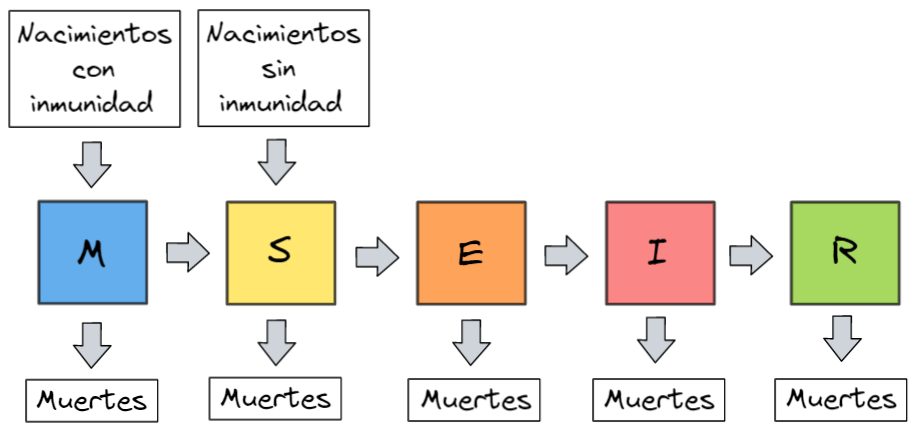
\includegraphics[width=0.6\textwidth]{Imagenes/MSEIR_compatimientos.PNG}
  \caption{Diagrama de compartimientos para el modelo MSEIR}
  \label{fig:MSEIR}
\end{figure}

Generalmente, cuando hablamos de modelos epidemiológicos se consideran tres estados o clases en las que podemos dividir a la población en el tiempo: Los que pueden contraer la enfermedad, los que se infectan y los que se recuperan. Si los que se recuperan no adquieren una inmunidad permanente, nos encontraremos ante un modelo SIS, en el que los susceptibles pueden contraer la enfermedad y una vez se recuperan vuelven al estado de susceptibilidad. Por otro lado, si los individuos que se recuperan generan inmunidad a la enfermedad, estaremos ante un modelo SIR. 

Teniendo en cuenta este tipo de consideraciones nos permitimos establecer a los modelos SIS y SIR como foco principal de nuestra investigación, sin dejar a un lado la idea de retomar modelos como el MSEIR en futuras investigaciones. Adicionalmente, para efectos aplicables consideraremos las variaciones que tienen en cuenta la natalidad y mortalidad bien sea a causa o por efectos ajenos a la enfermedad.

Brauer y Castillo describen en \cite{mateModelsInPopulationAndEpidemiology} los planteamientos y técnicas para analizar este tipo de modelos. Nos apoyaremos también en el trabajo realizado por Diego de Pereda Sebastián en \cite{diego2010} para algunos resultados y observaciones interesantes sobre cada modelo.

\subsection{El modelo SIS}\label{sub:modeloSIS}

El modelo SIS considera 2 posibles estados, susceptibles (S) e infectados (I). Las variaciones entre los estados vienen dadas por los nuevos contagios y los individuos que se recuperan de la enfermedad. Adicionalmente, cada estado se ve afectado por los parámetros que describen la natalidad/mortalidad y/o la muerte a causa de la enfermedad. 

Los diferentes estados del modelo se pueden apreciar en el diagrama (\ref{fig:SIS}):

\begin{figure}[h]
  \centering
    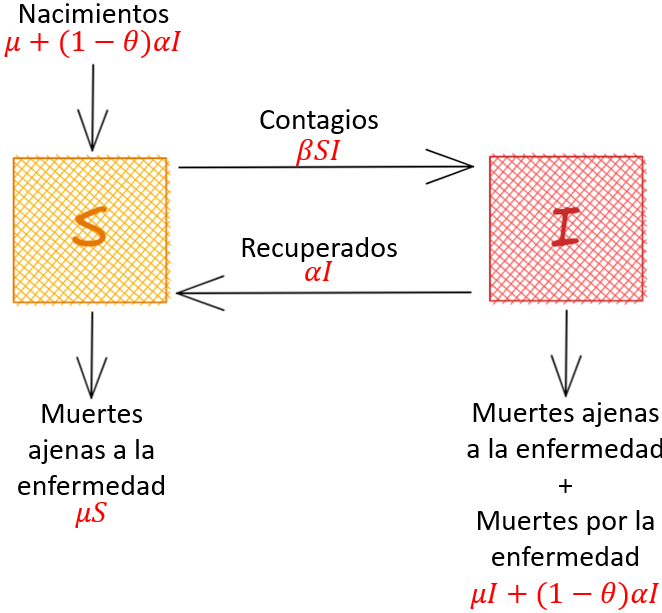
\includegraphics[width=0.4\textwidth]{Imagenes/SIS_compartimientos.PNG}
  \caption{Diagrama de compartimientos para el modelo SIS}
  \label{fig:SIS}
\end{figure}

Trabajaremos sobre una población de tamaño constante y normalizado, por lo que $S(t) + I(t) = 1$ y en consecuencia $S'(t) + I'(t) = 0$.

Normalmente, cuando se habla de modelos epidemiológicos con muerte por enfermedad se consideran 4 parámetros: 

\begin{itemize}
    \item La \textbf{tasa de infección $\beta$}, que representa la probabilidad que tiene un individuo susceptible de adquirir la enfermedad luego de tener contacto con un infectado.
    \item La \textbf{tasa de recuperación $\alpha$}, que podemos entender como la probabilidad de que un infectado se recupere de la enfermedad. En ocasiones representa el tiempo medio que tarda un infectado en recuperarse de la enfermedad \cite{diego2010}.
    \item La \textbf{tasa de natalidad/mortalidad $\mu$}, que en el caso de los modelos tradicionales se supone que son iguales. La natalidad nos indica la cantidad de individuos que ingresan al espacio y la mortalidad representa los individuos que fallecen por causas ajenas a la enfermedad.
    \item La \textbf{tasa de muerte por enfermedad $\theta$}, que nos indica la probabilidad que tiene un infectado de fallecer a causa de la enfermedad.
\end{itemize}

Podemos describir el modelo a partir de un sistema de ecuaciones diferenciales como sigue:

\begin{equation}\label{eq:modeloSIS}
\left\{
\begin{array}{l}
S' = \mu(1 - S) + (1 - \theta)\alpha I - \beta S I, \\
I' = \beta S I - (1 - \theta)\alpha I - \mu I.
\end{array}
\right.
\end{equation}

Para determinar los escenarios bajo los cuales una enfermedad es endémica, debemos calcular el valor de $\mathcal{R}_0$ para nuestro sistema de ecuaciones diferenciales (\ref{eq:modeloSIS}). Recuerde que para determinar el valor de $\mathcal{R}_0$ se considera una población completamente susceptible, es decir, $S=1$.

Observe que los nuevos infectados vienen dados por el término $\beta S$, con lo cual definimos $b(t) = \beta S = \beta$. Por otro lado, los flujos que determinan la salida del estado de infección de los individuos viene dado por los términos $-\alpha(1-\theta)I-\mu I$, de modo que si llamamos $I(t)$ a la cantidad de individuos infectados que permanecieron infectados desde el momento $t=0$, tenemos

\begin{equation}\label{eq:Cambio en I}
\frac{dI}{dt} = -\alpha(1-\theta)I-\mu I.
\end{equation}

Si usamos el método de separación de variables obtenemos

\begin{equation}\label{eq:Infectados en el tiempo}
I(t) = I(0)e^{-(\alpha(1-\theta)+\mu)t}.
\end{equation}

De ese modo, podemos afirmar que la proporción de individuos que permanecen infectados hasta un tiempo $t$ viene dado por $e^{-(\alpha(1-\theta)+\mu)t}$, con lo cual $F(t)=e^{-(\alpha(1-\theta)+\mu)t}$. Finalmente, al reemplazar en (\ref{eq:R0}) obtenemos:

\begin{align*}
\mathcal{R}_0 &= \lim_{T\to\infty}\int_0^T b(t)F(t) dt \\
&= \lim_{T\to\infty}\int_0^T \beta e^{-(\alpha(1-\theta)+\mu)t} dt\\
&= \frac{\beta}{\alpha(1-\theta)+\mu}.
\end{align*}

Una vez calculado el valor de $\mathcal{R}_0$, podemos reemplazar sobre la derivada para la población infectada de la ecuación (\ref{eq:modeloSIS}), con lo cual

\begin{align*}
    \frac{dI}{dt} &= \beta SI - \alpha(1-\theta)I - \mu I \\
    &= \left(S-\frac{1}{\mathcal{R}_0}\right)\beta I \\
    &< \left(1-\frac{1}{\mathcal{R}_0}\right)\beta I, \\
\end{align*}

de donde podemos afirmar que si $\mathcal{R}_0>1$, la derivada $I'$ será positiva, lo cual significa que la enfermedad será endémica. En el caso $\mathcal{R}_0<1$ nos encontraremos con una derivada negativa, por lo que la cantidad de infectados terminará desapareciendo, lo cual implica que la enfermedad no será endémica.

\subsubsection{Análisis de estabilidad}

Para analizar la estabilidad de nuestro modelo SIS debemos conocer sus puntos de equilibrio. Al anular ambas derivadas nos damos cuenta de que están dados por:

$$\begin{array}{ccc}
    P_0=(S_a,I_a)=(1,0) & \text{y} & P_1=(S_b,I_b)=\left(\frac{\alpha(1-\theta)+\mu}{\beta},\frac{\beta-\alpha(1-\theta)-\mu}{\beta}\right).
\end{array}$$

Veamos que los puntos de equilibrio pertenecen al conjunto de posibles soluciones de nuestro sistema, es decir, veamos que satisfacen las condiciones de tener coordenadas positivas y menores o iguales a 1:

En el caso de $P_0$ la verificación es trivial. Por otro lado, para el caso de $P_1$ observe que 

$$0\leq\alpha(1-\theta)+\mu\leq\beta \longrightarrow \frac{\alpha(1-\theta)+\mu}{\beta}\text{, }\frac{\beta+\alpha(1-\theta)+\mu}{\beta}\geq0.$$

Si dividimos la expresión del lado izquierdo por $\beta$ obtenemos:

$$0\leq \frac{\alpha(1-\theta)+\mu}{\beta}\leq1,$$

de donde podemos afirmar que 

$$1-\frac{\alpha(1-\theta)+\mu}{\beta}\leq1 \longrightarrow \frac{\beta-\alpha(1-\theta)-\mu}{\beta}\leq1.$$

De ese modo podemos concluir que ambos puntos de equilibrio cumplen las condiciones de tener coordenadas positivas y menores que la unidad.

Es momento de determinar los comportamientos que describen ambos puntos, $P_0$ y $P_1$. Para esto, considere el jacobiano de la parte lineal del sistema (\ref{eq:modeloSIS}) dado por:

$$|A-\lambda I|=
\left|\begin{array}{cc}
-\mu-\lambda & \alpha(1-\theta) \\
0 & -\alpha(1-\theta)-\mu-\lambda
\end{array}\right|.$$

De donde se obtienen los valores propios $\lambda_0 = -\mu$ y $\lambda_1 = -\alpha(1-\theta)-\mu$. Dado que $\mu$ representa la tasa de natalidad, $\alpha$ es la tasa de recuperación y $\theta$ es la probabilidad de morir a causa de la enfermedad, no puede ocurrir que $\mu,\alpha,\theta\leq0$, por lo que podemos afirmar que ambos puntos de equilibrio son hiperbólicos y, por otra parte, como claramente nuestro sistema es $C^1$, podemos aplicar el teorema de Hartman-Grobman, el cual nos garantiza que el sistema es conjugado topológicamente a su parte lineal en una vecindad abierta de cada uno de los puntos de equilibrio y de ese modo, concluimos que el sistema se comporta como un sumidero cerca de los puntos $P_0$ y $P_1$, concluyendo así la estabilidad de nuestro modelo en dichas vecindades.

\subsubsection{Estudio numérico}

Para representar las soluciones del sistema de ecuaciones diferenciales que describe el modelo SIS usaremos el método de Euler, el cual se implementó en el módulo:
\href{https://grupo-de-simulacion-con-automatas.github.io/CAsimulations-Modelacion-de-dinamicas-topologicas-en-la-propagacion-de-una-enfermedad-usando-CA/#:~:text=CellSpaceConfiguration-,CompartmentalModelsInEDOS,-Con\%20este\%20m\%C3\%B3dulo}{\underline{CompartimentalModels}} de la librería \href{https://github.com/Grupo-de-simulacion-con-automatas/Prediccion-del-comportamiento-de-una-enfermedad-simulada-en-AC-con-un-algoritmo-en-RN/tree/master/Codigo/CAsimulation}{CAsimulations} (\ref{CAsimulations}).

De manera general, dadas unas condiciones iniciales $S(0)=S_0,I(0)=I_0$ aplicamos el método de Euler a partir de la siguiente expresión:

$$\left\{\begin{array}{l}
S_{t+1} = S_t + h\cdot(\mu(1 - S_t) + (1 - \theta)\alpha I_t - \beta S_t I_t )\text{, y} \\
I_{t+1} = I_t + h\cdot(\beta S_t I_t - (1 - \theta)\alpha I_t - \mu I_t).
\end{array}\right.$$

El módulo \href{https://grupo-de-simulacion-con-automatas.github.io/CAsimulations-Modelacion-de-dinamicas-topologicas-en-la-propagacion-de-una-enfermedad-usando-CA/#:~:text=CellSpaceConfiguration-,CompartmentalModelsInEDOS,-Con\%20este\%20m\%C3\%B3dulo}{\underline{CompartimentalModels}} nos permite visualizar las soluciones para el modelo SIS dada una condición inicial, sin tener que recurrir a ninguna herramienta externa. Para esto debemos definir inicialmente a las funciones que describen las derivadas de nuestro modelo y luego las guardamos en una lista, como se muestra a continuación:

\begin{figure}[h]
    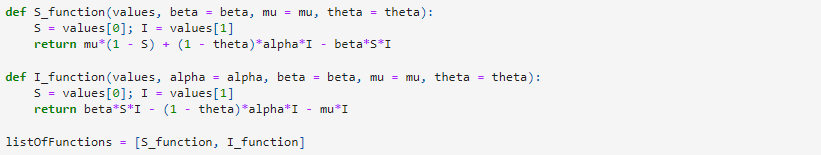
\includegraphics[width=1\textwidth]{Imagenes/compartimentalModels1.png}
\end{figure}

Si ahora suponemos que tenemos el caso de una enfermedad cuyos parámetros están dados por $\alpha=0.2$, $\beta=0.5$, $\theta=0.4$ y $\mu=\frac{1}{75\cdot365}$, obtendremos una gráfica como la de la figura (\ref{fig:Ejemplo 2 - SIS}) para las condiciones iniciales $S_0=0.9$ e $I_0=0.1$:

\begin{figure}[h]
    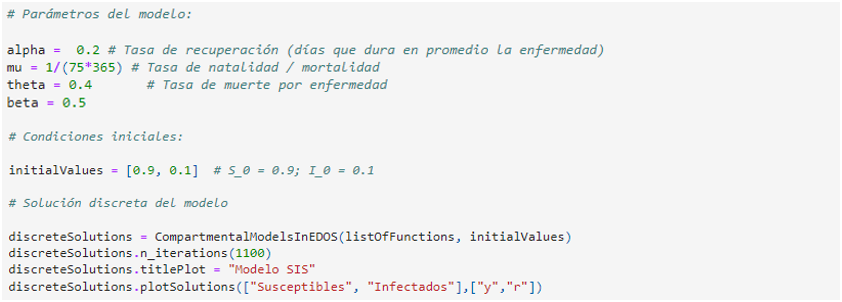
\includegraphics[width=1\textwidth]{Imagenes/compartimentalModels2.png}
\end{figure}
    
\begin{figure}[h]
  \centering
    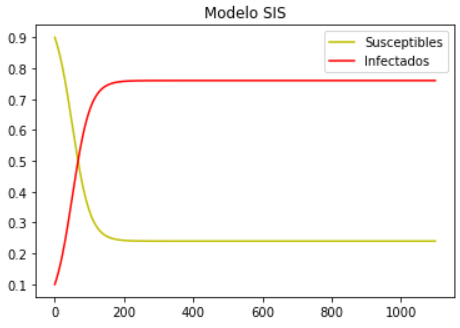
\includegraphics[width=0.45\textwidth]{Imagenes/ex1SIS.PNG}
  \caption{Evolución de la enfermedad en 1100 días ($h=0.1$).}
  \label{fig:Ejemplo 2 - SIS}
\end{figure}

%%%%%%%%%%%%%%%%%%%%%%%%%%%%%%%%%%%%%%%%%%%%%%%%%%%%%%%%%%%%%%%%%%%%%%%%%%%%%%%%%%%%%%%%%%%%%%%%
\newpage
%%%%%%%%%%%%%%%%%%%%%%%%%%%%%%%%%%%%%%%%%%%%%%%%%%%%%%%%%%%%%%%%%%%%%%%%%%%%%%%%%%%%%%%%%%%%%%%%

\subsection{El modelo SIR}\label{sub:modeloSIR}

Para este modelo se considera el estado de inmunidad (R) frente a la enfermedad. A diferencia del modelo SIS, en el modelo SIR no hay una interacción del estado I al estado S, ya que se supone que los individuos que se recuperen de la enfermedad no podrán volver a contraerla, por lo que pasaran al estado R. 

En el diagrama (\ref{fig:SIR}) se pueden apreciar las interacciones para los estados del modelo:

\begin{figure}[h]
  \centering
    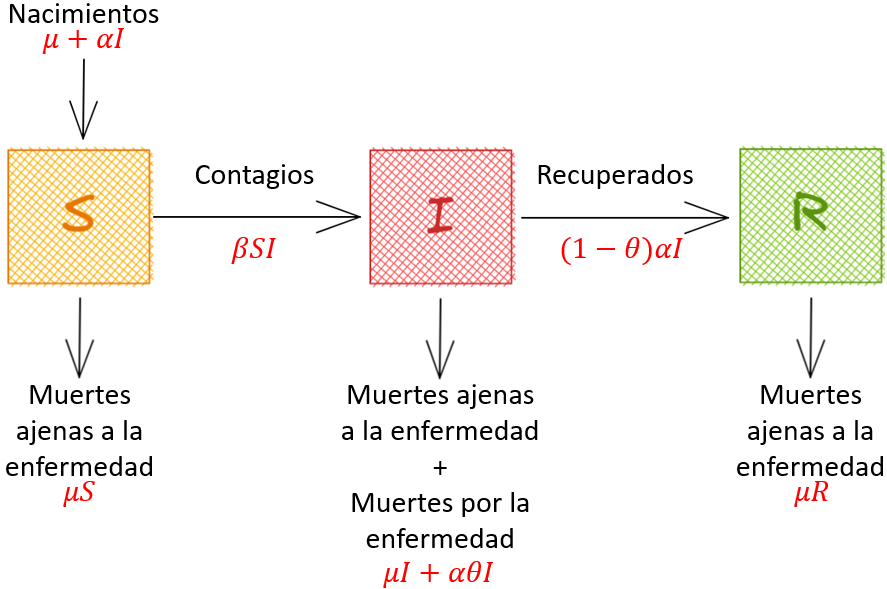
\includegraphics[width=0.75\textwidth]{Imagenes/SIR_compartimientos.PNG}
  \caption{Diagrama de compartimientos para el modelo SIR}
  \label{fig:SIR}
\end{figure}

El sistema de ecuaciones diferenciales que describe las interacciones entre estados viene dado por la siguiente ecuación:

\begin{equation}\label{eq:Modelo SIR}
\left\{
\begin{array}{l}
S' = \mu(1 - S) + \alpha\theta I - \beta S I, \\
I' = \beta S I - \mu I - \theta\alpha I - (1 - \theta)\alpha I = \beta S I - \alpha I - \mu I\text{, y } \\
R' = \alpha I - \alpha\theta I - \mu R.
\end{array}
\right.
\end{equation}

En este caso, la ecuación diferencial que describirá la cantidad de individuos infectados desde el momento 0 viene dada por:

\begin{equation}\label{eq:Infectados en el tiempo I - SIR}
    \frac{dI}{dt}=-\mu I - \alpha I \longrightarrow I(t)=I(0)e^{-(\alpha+\mu)t}.
\end{equation}

Con lo que definimos $F(t)=e^{-(\alpha+\mu)t}$. Por otra parte, la función $b(t)$ estará definida de la misma manera que en el modelo SIS debido a la manera en la que se describe el modelo. Así, al reemplazar en (\ref{eq:R0}):

\begin{align*}
\mathcal{R}_0 &= \int_0^\infty b(t)F(t) dt \\
&= \lim_{T\to\infty} \int_0^T b(t)F(t) dt \\
&= \frac{\beta}{\alpha+\mu}.
\end{align*}

\textit{Observación:} De acuerdo con la ecuación (\ref{eq:Infectados en el tiempo I - SIR}), la población de infectada tendera a cero cuando $t$ tienda a infinito.

De la derivada para la población infectada de la ecuación (\ref{eq:Modelo SIR}), podemos observar que:

\begin{align*}
    \frac{dI}{dt} &= \beta SI - \alpha I - \mu I \\
    &= \left(S-\frac{1}{\mathcal{R}_0}\right)\beta I \\
    &< \left(1-\frac{1}{\mathcal{R}_0}\right)\beta I, \\
\end{align*}

de donde podemos afirmar que si $\mathcal{R}_0>1$, la derivada $I'$ será positiva, lo cual significa que la enfermedad será endémica, mientras que si $\mathcal{R}_0<1$, la enfermedad terminará desapareciendo junto con la cantidad de infectados por iteración.

\subsubsection{Análisis de estabilidad}

Al igualar a cero las derivadas del sistema de ecuaciones (\ref{eq:Modelo SIR}) obtenemos los puntos de equilibrio:

$$\begin{array}{ccc}
P_0=(S_a,I_a,R_a)=(1,0,0) & \text{y} & P_1=(S_b,I_b,R_b)=\left(\frac{\alpha+\mu}{\beta},\frac{\mu(\beta-\alpha-\mu)}{\beta(\mu+(1-\theta)\alpha)},\frac{(1-\theta)\alpha(\beta-\alpha-\mu)}{\beta(\mu+(1-\theta)\alpha)}\right).
\end{array}$$

Veamos que las coordenadas de ambos puntos cumplen las condiciones de ser positivos y menores o iguales que uno: 

En el caso de $P_0$ se cumple de manera trivial. Por otro lado, como $\alpha,\beta,\theta$ y $\mu$ son valores positivos podemos afirmar que $S_b>0$, para $I_b$ y $R_b$ observe que 

$$\begin{array}{ccc}
\frac{\mu(\beta-\alpha-\mu)}{\beta(\mu+(1-\theta)\alpha)},\frac{(1-\theta)\alpha(\beta-\alpha-\mu)}{\beta(\mu+(1-\theta)\alpha)}>0 & \text{, si} & \beta-\alpha-\mu>0.
\end{array}$$

De la ecuación anterior podemos afirmar que 

$$\beta-\alpha-\mu>0\longrightarrow1>\frac{\alpha+\mu}{\beta}.$$

Además, como ya sabemos que se trata de un valor positivo podemos deducir que 

\begin{align*}
1&>1-\frac{\alpha+\mu}{\beta} \\
&= \frac{(\beta-\alpha-\mu)(\mu+(1-\theta)\alpha)}{\beta(\mu+(1-\theta)\alpha)}\\
&= \frac{\mu(\beta-\alpha-\mu)}{\beta(\mu+(1-\theta)\alpha)}+\frac{(1-\theta)\alpha(\beta-\alpha-\mu)}{\beta(\mu+(1-\theta)\alpha)}.
\end{align*}

Así,

$$\frac{\mu(\beta-\alpha-\mu)}{\beta(\mu+(1-\theta)\alpha)},\frac{(1-\theta)\alpha(\beta-\alpha-\mu)}{\beta(\mu+(1-\theta)\alpha)}<1.$$

Hemos demostrado que ambos puntos de equilibrio cumplen con las condiciones de tener coordenadas positivas y menores a la unidad. Ahora analizaremos los comportamientos que describen los puntos, $P_0$ y $P_1$. Para esto, considere el jacobiano de la parte lineal del sistema (\ref{eq:Modelo SIR}) dado por:

$$|A-\lambda I|=(-\mu-\lambda)
\left|\begin{array}{cc}
-\mu-\lambda & \theta\alpha\\
0 & -\alpha-\mu -\lambda
\end{array}\right|.$$

De donde se obtienen los valores propios $\lambda_0 = -\mu$ y $\lambda_1 = -\alpha-\mu$. Dado que $\mu$ representa la tasa de natalidad y $\alpha$ la tasa de recuperación, no puede ocurrir que $\mu,\alpha\leq0$, por lo que podemos afirmar que ambos puntos de equilibrio son hiperbólicos y, por otra parte, como claramente nuestro sistema es $C^1$, podemos aplicar el teorema de Hartman-Grobman de la misma manera a como se aplicó en la sección anterior, concluyendo así, que el sistema se comporta como un sumidero cerca de los puntos $P_0$ y $P_1$, concluyendo así la estabilidad de nuestro modelo en dichas vecindades.

% Ahora analizaremos la estabilidad de nuestro modelo SIR, consideremos el jacobiano de nuestro sistema de ecuaciones diferenciales:

% $$|A-\lambda I|=(-\mu-\lambda)
% \left|\begin{array}{cc}
% -\beta I-\mu-\lambda & -\beta S+\theta\alpha\\
% \beta I & \beta S-\alpha-\mu -\lambda
% \end{array}\right|.$$

% Si evaluamos en el punto $P_1$, podemos identificar un comportamiento de tipo silla si $\beta-\alpha-\mu>0$, en caso contrario nos encontraremos ante un nodo estable. Si tomamos ahora el punto $P_2$ y observamos los valores propios:

% $$\left\{\begin{array}{l}
% \lambda=-\mu,\\
% \lambda=-\frac{1}{2}\frac{\mu\beta-\mu\theta\alpha+\sqrt{(\mu\beta-\mu\theta\alpha)^2-4\mu(\beta-\alpha-\mu)(\alpha+\mu-\theta\alpha)^2}}{\alpha+\mu-\theta\alpha} \text{, y}\\
% \lambda=-\frac{1}{2}\frac{\mu\beta-\mu\theta\alpha-\sqrt{(\mu\beta-\mu\theta\alpha)^2-4\mu(\beta-\alpha-\mu)(\alpha+\mu-\theta\alpha)^2}}{\alpha+\mu-\theta\alpha}.
% \end{array}\right.$$

% De ese modo obtendremos dos tipos de comportamientos: una espiral estable si los valores propios son imaginarios y un nodo estable en el caso de que los valores propios sean reales.

\subsubsection{Estudio numérico}

De manera general, si usamos el método de Euler dadas las condiciones iniciales $S(0)=S_0,I(0)=I_0$ y $R(0)=R_0$ las expresiones que describen las soluciones discretas son:

$$\left\{\begin{array}{l}
S_{t+1} = S_t + h\cdot(\mu(1 - S_t) + \alpha\theta I_t - \beta S_t I_t), \\
I_{t+1} = I_t + h\cdot(\beta S_t I_t - \alpha I_t - \mu I_t)\text{, y} \\
R_{t+1} = R_t + h\cdot(\alpha I_t - \alpha\theta I_t - \mu R_t).
\end{array}\right.$$

Al igual que con el modelo anterior, nos apoyaremos sobre el módulo \href{https://grupo-de-simulacion-con-automatas.github.io/CAsimulations-Modelacion-de-dinamicas-topologicas-en-la-propagacion-de-una-enfermedad-usando-CA/#:~:text=CellSpaceConfiguration-,CompartmentalModelsInEDOS,-Con\%20este\%20m\%C3\%B3dulo}{\underline{CompartimentalModels}} para visualizar las soluciones del modelo SIR, con lo cual debemos definir inicialmente nuestro sistema de ecuaciones, esto es:

\begin{figure}[h]
  \centering
    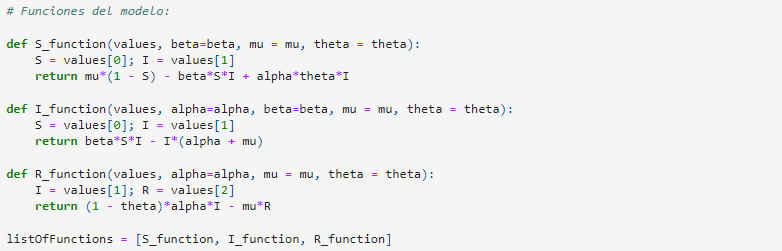
\includegraphics[width=1\textwidth]{Imagenes/compartimentalModels3.png}
\end{figure}

Si suponemos una enfermedad con los mismos parámetros del ejemplo que usamos para el modelo SIS, con la diferencia de que los individuos que se recuperan ganan inmunidad frente a la enfermedad, obtendremos algo como lo que se puede apreciar en la figura (\ref{fig:Ejemplo 2 - SIR}) para las condiciones $S_0=0.9,I_0=0.1,R_0=0$.

%%%%%%%%%%%%%%%%%%%%%%%%%%%%%%%%%%%%%%%%%%%%%%%%%%%%%%%%%%%%%%%%%%%%%%%%%%%%%%%%%%%%%%%%%%%%%%%%
% \newpage
%%%%%%%%%%%%%%%%%%%%%%%%%%%%%%%%%%%%%%%%%%%%%%%%%%%%%%%%%%%%%%%%%%%%%%%%%%%%%%%%%%%%%%%%%%%%%%%%

\begin{figure}[h]
  \centering
    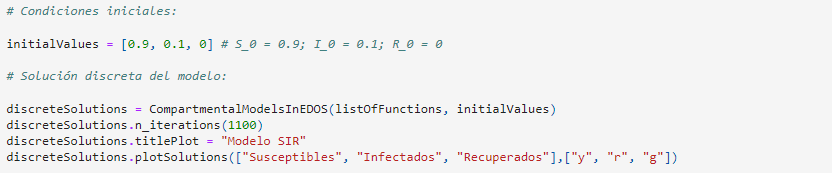
\includegraphics[width=1\textwidth]{Imagenes/compartimentalModels4.png}
\end{figure}

\begin{figure}[h]
  \centering
    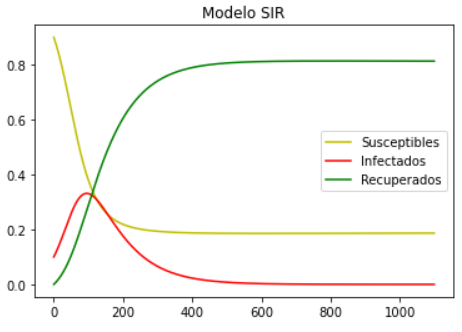
\includegraphics[width=0.45\textwidth]{Imagenes/ex1SIR.PNG}
  \caption{\centering Evolución de la enfermedad en 1100 días con ($h=0.1$).}
  \label{fig:Ejemplo 2 - SIR}
\end{figure}


\section{Algunos conceptos de topología}\label{sec:NocionesTopología}

Empezaremos esta sección con algunas definiciones y propiedades básicas de topología, pasando por conceptos como el de base y de vecindad para luego exponer dos proposiciones para la construcción de topologías a partir de sub colecciones de la familia de partes de un conjunto y finalmente hablaremos de propiedades de orden y numerabilidad para el enfoque de nuestro proyecto. Para esto nos apoyaremos en los conceptos expuestos por Munkres en \cite{munkres}, Casarrubias y Tamariz en \cite{elementosTopologiaGeneral}, Macho en \cite{stadler2002}, Neira en \cite{NeiraNacional} y Barmak en \cite{barmak2011}.

\begin{definition}\label{def:topologia}
Una \textit{topología} sobre un conjunto $X$ es una colección $\tau$ de subconjuntos de $X$ que satisface las siguientes condiciones:
\begin{enumerate}
    \item $\emptyset$ y $X$ están en $\tau$,
    \item si $A,B\in\tau$, entonces $A\cap B\in\tau$, y 
    \item la unión de cualquier subcolección de $\tau$ esta en $\tau$.
\end{enumerate}
Los elementos de $\tau$ se conocen como \textit{abiertos} de $X$ y la pareja $(X,\tau)$ es llamada como un \textit{espacio topológico}. Es común encontrar menciones a $X$ como un espacio topológico, esto se hace solo si el contexto es lo suficientemente claro como para omitir a $\tau$ de la escritura.
\end{definition}

\begin{example}\label{ex:topologíaDiscreta} 
Observe que para $X$ un conjunto cualquiera, la familia de todos los subconjuntos de $X$ es una topología sobre $X$. Esta topología se conoce como la \textit{topología discreta} de $X$.
\end{example}

\begin{example}\label{ex:exBase}
Considere al conjunto $X=\{a,b,c\}$ y a una sub-colección $\mathcal{A}$ de $X$ definida como: 
$$\mathcal{A}=\{\emptyset,\{a\},\{b\}.\{a,b\},\{a,c\},\{a,b,c\}\}.$$
Veamos que la colección $\mathcal{A}$ es una topología sobre $X$:
\begin{enumerate}
    \item Por la definición de $\mathcal{A}$ sabemos que $\emptyset$ y $X$ hacen parte de sus elementos.
    \item Si calculamos todas las posibles intersecciones obtendremos los siguientes conjuntos:
    $$\begin{array}{cccccc}
        \emptyset, & \{a\}, & \{b\}, & \{a,b\}, & \{a,c\}.
    \end{array}$$
    Como cada posible intersección está en el conjunto $\mathcal{A}$, podemos concluir que se cumple la segunda condición de la definición de topología.
    \item Al calcular todas las posibles uniones de sub-colecciones de $\mathcal{A}$ obtendremos los siguientes conjuntos:
    $$\begin{array}{cccccc}
        \{a\}, & \{b\}, & \{a,b\}, & \{a,c\}, & \{a,b,c\}.
    \end{array}$$
    De la misma manera que en el item anterior, de la definición de $\mathcal{A}$ se concluye la tercera condición y de ese modo se afirma que $\mathcal{A}$ es una topología sobre $X$.
\end{enumerate}
\end{example}

En ocasiones describir específicamente la topología de un conjunto es una tarea bastante compleja. Para evitar este tipo de inconvenientes se especifica una colección más pequeña de subconjuntos de $X$ llamada base de la topología sobre $X$, que es capaz de definir dicha topología. 

\begin{definition}\label{def:base}
Una \textit{base} para una topología sobre un conjunto $X$ es una colección $\mathcal{B}$ de subconjuntos de $X$ tales que:
\begin{enumerate}
    \item Para todo $x\in X$, existe $B\in\mathcal{B}$ tal que $x\in B$, y
    \item dados $B_1,B_2\in\mathcal{B}$, existe $B_3\in\mathcal{B}$ tal que $B_3\subseteq B_1\cap B_2$.
\end{enumerate}
Los elementos de $\mathcal{B}$ son llamados elementos básicos de $\mathcal{B}$.
\end{definition}

\begin{example}\label{ex:conUnipuntuales}
La colección de las uniones de conjuntos uni-puntuales de cualquier conjunto $X$, forma una base para la topología discreta de $X$.
\end{example}

A continuación definiremos uno de los conceptos que más usaremos a lo largo del presente documento. Usualmente, la vecindad de un elemento se entiende como el conjunto de los puntos ''cercanos'' (en el caso de espacios métricos) o en general, con los que podría tener algún tipo de relación. 

\begin{definition}\label{def:vecindad}
Sean $X$ un espacio topológico y $x\in X$. Diremos que un subconjunto $V$ de $X$ es una \textit{vecindad} de $x$, si existe un abierto $A$ tal que $x\in A\subseteq V$. Denotaremos por $\mathcal{V}(x)$ a la familia de todas las vecindades de $x$.
\end{definition}

\begin{example}\label{ex:sisVecindades}
Identificaremos al conjunto de vecindades $\mathcal{V}(a)$ para el punto $a$ del conjunto $X$ definido en el ejemplo \ref{ex:exBase}. Esto es:
$$\mathcal{V}(a)=\{\{a\},\{a,b\},\{a,c\},\{a,b,c\}\}$$
\end{example}

La definición anterior nos permite realizar la siguiente afirmación:

\begin{teorema}\label{teo:abiertoImplicaVecindad}
Un subconjunto $A$ de un espacio topológico $X$ es un conjunto abierto si, y solo si es vecindad de cada uno de los puntos que contiene.
\end{teorema}
\begin{proof}
La primera implicación se obtiene del hecho de que $A$ es abierto y $A\subseteq A$. Por otra parte, si suponemos que $A$ es vecindad de cada uno de sus puntos podemos afirmar que para cada $x\in A$ existe un abierto $V_x$ tal que $x\in V_x\subseteq A$. Veamos que $A=\bigcup_{x\in A}V_x$:

$(\supseteq)$ Se obtiene de manera trivial por la definición de los conjuntos $V_x$.

$(\subseteq)$ Sea $x\in A$. Ya que $A$ es vecindad de cada uno de sus puntos existe $V_x$ tal que $x\in V_x\subseteq A$, de modo que $x\in V_x\subseteq\bigcup_{x\in A}V_x$. Con lo que concluimos la igualdad.
\end{proof}

En la siguiente proposición se exponen las propiedades que poseen las familias de vecindades.

\begin{proposicion}\label{pro:propiedadesSistemaVecindades}
Sea $X$ un espacio topológico, entonces para cada $x\in X$:
\begin{enumerate}
    \item Si $U\in\mathcal{V}(x)$, entonces $x\in U$,
    \item si $U,V\in\mathcal{V}(x)$, entonces $U\cap V\in\mathcal{V}(x)$,
    \item para cada $U\in\mathcal{V}(x)$, existe $V\in\mathcal{V}(y)$ tal que $U\in\mathcal{V}(y)$ para cada $y\in V$, y 
    \item si $U\in\mathcal{V}(x)$ y $U\subseteq V\subseteq X$ entonces $V\in\mathcal{V}(x)$.
\end{enumerate}
\end{proposicion}

\begin{proof} $$$$
\begin{enumerate}
    \item Se verifica directamente de la definición de vecindad. 
    \item Sean $A,B\in\tau$ tales que $x\in A\subset U$ y $x\in B\subset V$, luego $x\in A\cap B\subseteq U\cap V$, con $A\cap B\in\tau$. De ese modo, por la definición de vecindad se concluye que $U\cap V\in\mathcal{V}(x)$.
    \item Sea $U\in\mathcal{V}(x)$. Entonces existe $V\in\tau$ tal que $x\in V\subseteq U$.
    
    Dado que $V$ es abierto, por el Teorema 2.4.6 se cumple que $V\in\mathcal{V}(x)$. Además, si $y\in V$ entonces $y\in V\subseteq U$ y $V\in\tau$ por lo que $U\in\mathcal{V}(y)$ para $y\in V$ arbitrario.
    \item Sea $U\in\mathcal{V}(x)$, luego existe $A\in\tau$ tal que $x\in A\subseteq V$, además como $A\in\mathcal{\tau}$ aplicamos la definición de vecindad y tenemos $V\in\mathcal{V}(x)$.
\end{enumerate} 
\end{proof}

Así como una base de una topología $\tau$ contiene toda la información necesaria para generarla, podemos tomar de manera conveniente alguna subcolección de $\mathcal{V}(x)$ que guarde la información topológica necesaria para generar a $\mathcal{V}(x)$. La siguiente definición nos permite determinar cuáles serían los componentes necesarios para formar al conjunto $\mathcal{V}(x)$.

\begin{definition}\label{def:sistemaFundamentalVecindades}
Para un punto $x$ en un espacio topológico $X$, un subconjunto $\mathcal{B}(x)$ de $\mathcal{V}(x)$ es un \textit{sistema fundamental de vecindades de $x$} sí para cada $V\in\mathcal{V}(x)$, existe $B\in\mathcal{B}(x)$ tal que $B\subseteq V$. Los elementos de $\mathcal{B}(x)$ son llamados \textit{vecindades (o entornos) básicos} de $x$.
\end{definition}

\begin{example}\label{ex:sistemaFundamentalVecindades}
Del ejemplo \ref{ex:exBase} podemos identificar los siguientes sistemas fundamentales de vecindades:
\begin{align*}
    \mathcal{B}(a) &= \{\{a\},\{a,b\},\{a,c\}\},\\
    \mathcal{B}(b) &= \{\{a,b\},\{a,b,c\}\}\text{, y }\\
    \mathcal{B}(c) &= \{\{a,c\},\{a,b,c\}\}.
\end{align*}
\end{example}

La definición \ref{def:sistemaFundamentalVecindades} nos motiva a pensar en los métodos para contruir topologías sobre un conjunto $X$ con propiedades particulares. A continuación mostraremos dos de ellos:

\begin{proposicion}\label{pro:topologiaGenerada1}
Sea $\mathcal{B}$ una familia de subconjuntos de un conjunto $X$ que satisface:
\begin{enumerate}
    \item $X=\bigcup \mathcal{B}$, y 
    \item si $B_1,B_2\in\mathcal{B}$ y $x\in B_1\cap B_2$, entonces existe $B\in\mathcal{B}$ tal que $x\in B\subseteq B_1\cap B_2$.
\end{enumerate}
Entonces la colección $\tau_\mathcal{B}=\{A\subseteq X:\exists\mathcal{A}\subseteq\mathcal{B}\text{ con }A=\bigcup\mathcal{A}\}$ es una topología sobre $X$ que contiene a $\mathcal{B}$ como base.
\end{proposicion}
\begin{proof}
Claramente $\emptyset$ y $X$ estan en $\tau_\mathcal{B}$. Considere ahora los conjuntos $A_1,A_2\in\tau_\mathcal{B}$ y veamos que su interesección es un elemento en $\tau_\mathcal{B}$: Si $A_1\cap A_2=\emptyset$ la propiedad se deduce del caso anterior. Supongamos que $A_1\cap A_2\neq\emptyset$, luego para $x\in A_1\cap A_2$ existen $B_1,B_2\in\mathcal{B}$ tales que $x\in B_1\cap B_2$ y $B_1\subseteq A_1, B_2\subseteq A_2$ con $A_i=\bigcup B_i$ para $B_i\in\mathcal{B}$ e $i\in\{1,2\}$. Así, de (2) podemos afirmar que existe $B_x\in\mathcal{B}$ tal que $B_x\subseteq B_1\cap B_2$. De manera análoga a la demostración de la igualdad de conjuntos del teoréma 1.4.6 podemos afirmar que: 
$$A_1\cap A_2=\bigcup\{B_x:x\in A_1\cap A_2\}.$$
Para demostrar el inciso 3 en la Definición 2.4.1 considere una subcolección $\mathcal{A}\subset\tau_\mathcal{B}$ y observe que
\begin{align*}
    \bigcup\mathcal{A} &= \bigcup\{A:A=\bigcup\mathcal{C}\text{ con }A\in\mathcal{A}\text{ y }\mathcal{C}\subseteq\mathcal{B}\}\\
    &= \bigcup\{\bigcup\mathcal{C}:\bigcup\mathcal{C}\in\mathcal{A}\text{ y }\mathcal{C}\subseteq\mathcal{B}\}\\
    &= \bigcup\{\mathcal{C}:\bigcup\mathcal{C}\in\mathcal{A}\text{ y }\mathcal{C}\subseteq\mathcal{B}\}.
\end{align*}
Por lo tanto $\bigcup\mathcal{A}\in\tau_\mathcal{B}$.
\end{proof}

\begin{proposicion}\label{pro:topologiaGenerada2}
Si para cada $x\in X$ se elige una familia $\mathcal{V}(x)\neq\emptyset$  de subconjuntos de $X$ de tal forma que las colecciones $\mathcal{V}(x)$ cumplen:
\begin{enumerate}
    \item Si $U\in\mathcal{V}(x)$, entonces $x\in U$,
    \item si $U,V\in\mathcal{V}(x)$, entonces $U\cap V\in\mathcal{V}(x)$,
    \item para cada $U\in\mathcal{V}(x)$, existe $V\in\mathcal{V}(x)$ tal que $U\in\mathcal{V}(y)$ para cada $y\in V$, y 
    \item Si $U\in\mathcal{V}(x)$ y $U\subseteq V\subseteq X$, entonces $V\in\mathcal{V}(x)$,
\end{enumerate}
entonces la familia $\tau=\{\emptyset\}\cup\{A\subseteq X:\text{para cada }x\in A\text{ existe }V\in\mathcal{V}(x)\text{ con }V\subseteq A\}$ es un sistema de vecindades de $x$ para esta topología.
\end{proposicion}
\begin{proof}
Demostraremos primero que $\tau$ es una topología: Por la definición de $\tau$ tenemos $\emptyset\in\tau$. Si tomamos $x\in X$ sabemos que existe $U\in\mathcal{V}(x)$, en particular $U\subseteq X$ y de ese modo $X\in\tau$. Considere ahora $A_1,A_2\in\tau$ y $x\in A_1\cap A_2$, luego por hipotésis existen $U_1,U_2\in\mathcal{V}(x)$ tales que $x\in U_1\subseteq A_1$ y $x\in U_2\subseteq A_2$. Del inciso (2) se tiene que $U_1\cap U_2\in\mathcal{V}(x)$ y como $x\in A_1\cap A_2$ se afirma que $U_1\cap U_2\subseteq A_1\cap A_2\in\tau$. Para mostrar el (3) inciso de la definición de topología, considere $\mathcal{A}\subseteq\tau$ y $x\in\bigcup\mathcal{A}$, entonces existe $A\in\mathcal{A}$ tal que $x\in A$. Como $A\in\tau$ existe $U\in\mathcal{V}(x)$ tal que $x\in U\subseteq A$. De lo anterior y del hecho de que $U\subseteq\bigcup\mathcal{A}$, concluimos que $\bigcup\mathcal{A}\in\tau$ y por lo tanto $\tau$ es una topología sobre $X$.

Para demostrar que $\mathcal{V}(x)$ es el sistema fundamental de vecindades veamos primero que es una familia de vecindades: Tome $U\in\mathcal{V}(x)$ y $A=\{y\in U:U\in\mathcal{V}(y)\}\in\tau$. Luego, para $a\in A$ se cumple que $a\in U$ y $U\in\mathcal{V}(a)$. De la condición (3) se sabe que existe $V_a\in\mathcal{V}(a)$ tal que $U\in\mathcal{V}(y)$ para cada $y\in V_a$. De la definición de $A$ se cumple que $V_a\subseteq A$ y de la cuarta condición podemos afirmar que $A\in\mathcal{V}(a)$, con lo cual $A\in\tau$. Se concluye que $U$ es vecindad de $x$ y $\mathcal{V}(x)$ es una familia de vecindades de $x$.

Finalmente, para una vecindad $U$ de $x$ existe $V\in\tau$ tal que $x\in V\subseteq U$ por la definición de vecindad. Luego $V\in\mathcal{V}(x)$ y así, $\mathcal{V}(x)$ es sistema fundamental de vecindades en $(X,\tau)$.
\end{proof}

Es natural pensar en que si consideramos un sistema de vecindades $\mathcal{V}(x)$, se establezca una relación de orden parcial con los demás elementos. Teniendo esto en mente definimos los siguientes conceptos:

\begin{definition}\label{def:vecindadMinimal}
Una \textit{vecindad minimal de} $x$ es la intersección de todas las vecindades de $x$. Lo denotaremos como $U_x$.
\end{definition}

\begin{example}\label{ex:vecindadMinimalEnUnipuntuales}
En la topología discreta las vecindades minimales coinciden con los conjuntos unipuntuales.
\end{example}

\begin{example}\label{ex:minimalesExBase}
Si concideramos la topología $\mathcal{A}$ y el espacio $X$ del ejemplo \ref{ex:exBase}. Las vecindades minimales son:
$$U_a = \{a\}\text{, }U_b = \{b\}\text{ y }U_c=\{a,c\}.$$
\end{example}

\begin{proposicion}\label{pro:baseMinimal}
La unión de todas las vecindades minimales $U_x$ para $x\in X$ forma una base para la topología de $X$. Esta base es llamada \textit{base minimal}.
\end{proposicion}

Es facil ver que cualquier otra base de la topología sobre $X$ continene a la base minimal y esto a su vez garantiza que es una base para lo topología.

Los siguientes conceptos nos permiten determinar de manera formal cuales son las propiedades que definen un preorden finito y posteriormente una vecindad máximal de algún elemento.

\begin{definition}\label{def:conjuntoPreordenadoFinito}
Un \textit{conjunto preordenado finito} es un conjunto finito con una relación transitiva y reflexiva. Definiremos el la relación de orden parcial $x\preceq y$ si $x\in U_y$.
\end{definition}

\begin{definition}\label{def:maximal}
Un elemento $x$ en un conjunto parcialmente ordenado es llamado un maximal si $y\succeq x$ implica $y=x$, y es un máximo si $y\preceq x$ para todo $y\in X$.
\end{definition}

\begin{example}\label{ex:maximalesExBase}
Si retomamos el ejemplo \ref{ex:minimalesExBase} podremos determinar que los elementos $a$ y $b$ son maximales pero no comparables bajo el preorden $\preceq$. En particular $c\preceq a$ y $c\preceq b$.
\end{example}

Usualmente, al trabajar con espacios topológicos finitos se habla de los axiomas de numerabilidad. Para los objetivos de nuestro proyecto únicamente abordaremos el primero de ellos debido a que los demás solo se cumplen en algunos casos pasos particulares de nuestra investigación. Se espera profundizar más al rededor de estos casos específicos en futuras investigaciones.

\begin{definition}\label{def:espacio1Numerable}
Un espacio topológico $X$ que tiene un sistema fundamental de vecindades numerable en cada uno de sus puntos se dice que satisface el primer axioma de numerabilidad o simplemente que es uno-numerable.
\end{definition}

\begin{example}\label{ex:finito1Numerable}
Todo espacio topológico finito es un espacio uno-numerable.
\end{example}

\section{Autómatas celulares}\label{sec:Autómatas celulares}

Los autómatas celulares nacen con el trabajo de Von Neumann a finales de la década de 1940 con su trabajo \textit{``The General and Logical Theory of Automata"} en el que se plantean por primera vez las ideas para una máquina capaz de autorreplicarse. Trabajó sobre un sistema bidimensional discreto para desarrollar dinámicas bastante complejas que además fueran autorreplicables \cite{alfons2010,ACaplicacionesComputacion}.

De acuerdo con \cite{descripcionyAplicaciones}, podemos pensar en un autómata celular como un conjunto de células que tienen diferentes comportamientos en el tiempo y que interactúan entre sí, de la misma manera que en sistema biológico de donde se obtiene su nombre.

La implementación computacional de un autómata celular por lo general se hace sobre matrices o tensores, por lo que el sistema que se quiere modelar se describe sobre una malla de tamaño regular, como en la figura (\ref{fig:AC a matriz}). Una vez se definen las características de cada célula y sus relaciones con las demás, se establece una equivalencia con un conjunto de valores o caracteres que conoceremos como estados del autómata y finalmente, sobre esos estados definiremos las reglas de comportamiento para nuestro modelo.

\begin{figure}[h]
  \centering
    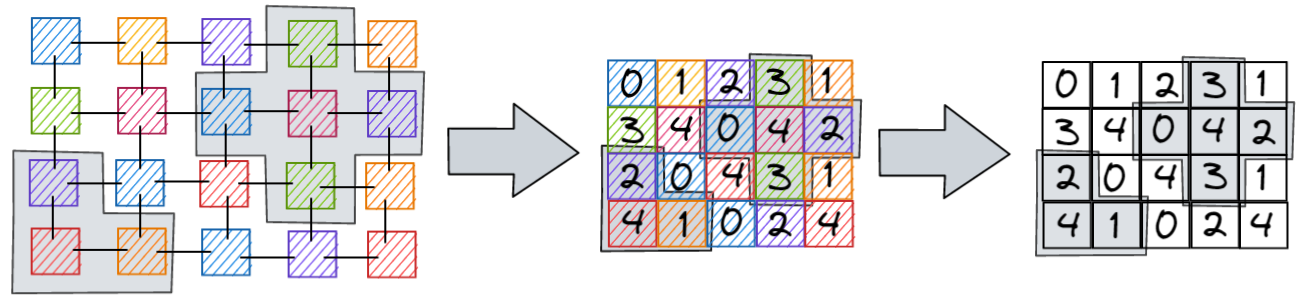
\includegraphics[width=1\textwidth]{Imagenes/ACaMatriz.PNG}
  \caption{Implementación computacional clásica de un autómata celular}
  \label{fig:AC a matriz}
\end{figure}

A continuación definiremos los elementos que componen a un autómata celular:

\subsubsection{Espacio de células}

Un espacio de células $\mathcal{L}$ es el conjunto donde viven e interactuan todas las células que se consideran para el modelo. En general este espacio es discreto, regular y finito, esto último debido a las limitaciones computacionales presentes en las herramientas con las que se construyen los modelos en autómatas celulares.

La condición de regularidad de nuestro espacio de células se refiere a que las celdas que lo conforman se organizan de una manera regular, con lo que podemos dotar al espacio $\mathcal{L}$ de una dimensión de la forma $n_1\times\cdots\times n_m$ para $n_1,\cdots,n_m\in\mathbb{Z}$.

\begin{proposicion}\label{pro:LEsEnumerable}
Todo espacio de células es un conjunto enumerable.
\end{proposicion}

La demostración de esta proposición se deduce directamente de la definición de espacio de células.

\textit{Nota:} En adelante cuando hablemos de un espacio de células se asumira que el espacio es bidimensional a menos que se indique lo contrario.

La implementación computacional de estos espacios nos permite definir condiciones de frontera que resultan bastante utiles para diferentes aplicaciones. Usualmente se consideran los siguientes tipos de borde:

\begin{itemize}
    \item \textbf{Bordes periódicos:} Las células opuestas son vecinas, es decir, $\mathcal{L}$ es un toro.
    \item \textbf{Bordes absorbentes:} Las células de los bordes no tienen vecinos fuera de los límites. En este caso $\mathcal{L}$ se puede entender como una región rectangular.
    \item \textbf{Bordes reflejantes:} Las células de los bordes tienen como vecinos fuera de los límites a la celda misma, formando una especie de espejo.
\end{itemize}

\begin{figure}[h]
  \centering
    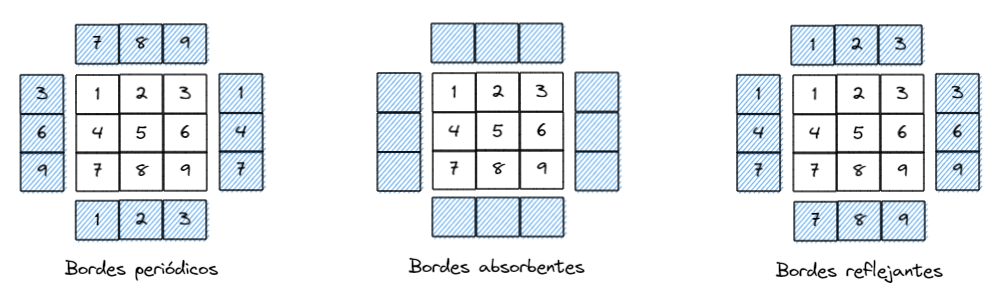
\includegraphics[width=0.8\textwidth]{Imagenes/Tipos_de_borde.PNG}
  \caption{Tipos de borde usuales para autómatas celulares}
  \label{fig:Tipos de borde}
\end{figure}
    
\textit{Nota:} Para los objetivos del proyecto implementaremos unicamente bordes del tipo absorbente.

\subsubsection{Conjunto de estados}

Dependiendo del contexto en que estemos implementando nuestro autómata celular, las células podrán adquirir diferentes atributos. Por ejemplo, si consideramos el ejercicio realizado en  \cite{NetLogoFireModel} en el que se modela la propagación del fuego en un bosque se consideran dos estados: los arboles que están quemados de color rojo y los que no se quemaron verde en la figura (\ref{fig:Fuego Netlogo}). Como puede apreciarse en el ejemplo, hay células que cambian de estado en el tiempo.

\begin{figure}[h]
  \centering
    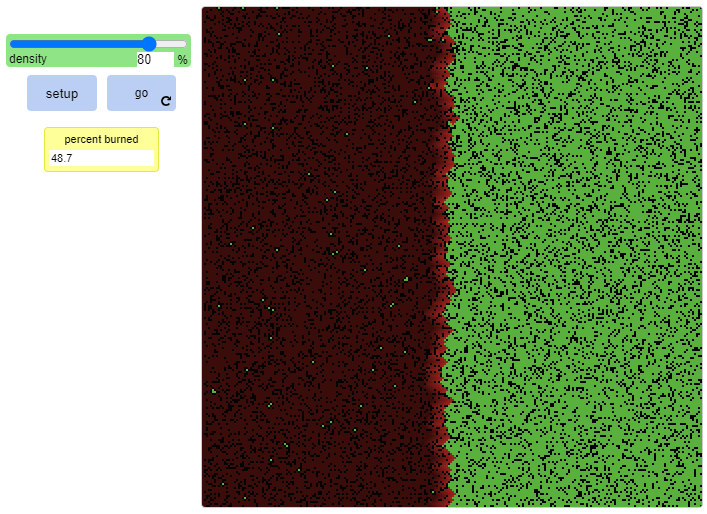
\includegraphics[width=0.4\textwidth]{Imagenes/netlogoEx1.PNG}
  \caption{Modelo del fuego en Netlogo. Captura tomada de \cite{NetLogoFireModel}.}
  \label{fig:Fuego Netlogo}
\end{figure}

\begin{definition}\label{conjuntoDeEstados}
El \textit{conjunto de estados} $\Sigma$ es el conjunto finito de todas las posibles categorias en las que pueden estar las células del espacio $\mathcal{L}$. Cada elemento $\sigma$ de $\Sigma$ será conocido como un estado del modelo.
\end{definition}

\subsubsection{Vecindades}

Una de las ventajas de trabajar con autómatas celulares es que permiten establecer relaciones entre las células por medio de vecindades. En general no se trabaja con todo el conjunto $\mathcal{V}(x)$ sino que se consideran elementos de cada una de estas familias para conformar un conjunto de vecindades sobre el espacio $\mathcal{L}$. Este conjunto se conoce como un \textit{sistema de vecindades} sobre $\mathcal{L}$.

Generalmente cuando se desarrollan análisis usando autómatas celulares se trabaja con sistemas de vecindades definidos a partir de las vecindades de Moore o de la de Von neumann. 

La vecindad de Von neumann se compone de una célula central y de las que se encuentran a los lados formando así una especie de cruz. De manera formal la vecindad de Von neumann de la celda $i,j$ se define como:

$$\mathcal{V}_V(x_{i,j}) = \{x_{k,l}\mid\abs{i-k}+\abs{j-l}\leq1\text{, con }k,l\in\mathbb{Z}\}$$

Por otro parte, tenemos a la vecindad de Moore la cual se define de manera similar a la vecindad de Von neumann. La diferencia entre una y otra radica en que la vecindad de Moore incluye a las células de las diagonales formando un cuadrado. La vecindad de Moore se define  de la célula $i,j$ como:

$$\mathcal{V}_M(x_{i,j}) = \{x_{k,l}\mid\abs{i-k},\abs{j-l}\leq1\text{, con }k,l\in\mathbb{Z}\}$$

En la figura (\ref{fig:Moore - Von neumann}) podemos identificar a las celdas de color verde como las células centrales correspondientes a las ubicadas en la posición $i,j$ para cada vecindad y las de color azul como sus vecinos:

\begin{figure}[h]
  \centering
    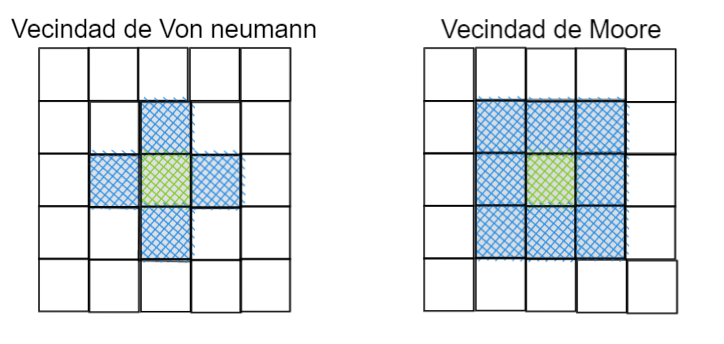
\includegraphics[width=0.5\textwidth]{Imagenes/vecindades.PNG}
  \caption{Vecindades usuales para autómatas celulares}
  \label{fig:Moore - Von neumann}
\end{figure}

%%%%%%%%%%%%%%%%%%%%%%%%%%%%%%%%%%%%%%%%%%%%%%%%%%%%%%%%%%%%%%%%%%%%%%%%%%%%%%%%%%%%%%%%%%%%%%%%%%
%\newpage
%%%%%%%%%%%%%%%%%%%%%%%%%%%%%%%%%%%%%%%%%%%%%%%%%%%%%%%%%%%%%%%%%%%%%%%%%%%%%%%%%%%%%%%%%%%%%%%%%%

\subsubsection{Reglas de evolución}

Las reglas de evolución definen la manera en la que cambian los estados de cada célula teniendo en cuenta el estado de sus vecinos. En general definimos una regla de evolución $\phi$ como sigue:

$$\phi:\Sigma_x\times\overbrace{\Sigma\times\Sigma\times\cdots\times\Sigma}^{N}\longrightarrow\Sigma_x,$$

donde $N$ es la cantidad de vecinos de $x$ y $\Sigma_x$ el conjunto de estados que puede tomar $x$. 

Para determinar la evolución del espacio $\mathcal{L}$ se debe aplicar la regla de evolución simultáneamente sobre cada una de sus células. De ese modo podemos definir una regla global de evolución $\Phi$ como la aplicación de la regla $\phi$ sobre cada una de las células de un espacio $\mathcal{L}$.

Las reglas de evolución pueden ser de dos tipos:

\begin{itemize}
    \item \textbf{Reglas determinísticas}
    
    Son aquellas en las que se define un estado para cada posible combinación de estados en la vecindad. Un ejemplo de esto son las \textbf{reglas de Wolfram}, en las que se define la correspondencia entre los estados de una celda $x$ y sus vecinos con el estado posterior de la celda $x$. Consideremos como caso particular a la regla 30 en la que se define la siguiente correspondencia:
    
    \begin{figure}[h]
      \centering
        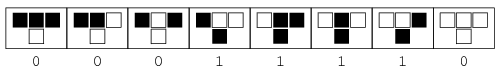
\includegraphics[width=0.7\textwidth]{Imagenes/regla30.PNG}
      \caption{Regla 30. Captura tomada de \cite{rule30}}
      \label{fig:Regla30}
    \end{figure}
    
    \newpage
    
    Al tratarse de una regla sobre un espacio 1-dimensional, los vecinos de cada célula son los que se encuentran a lados izquierdo y derecho, como se ve en la figura (\ref{fig:Regla30}). En este caso el conjunto de estados es de la forma $\Sigma=\{0,1\}$. En la siguiente figura podemos apreciar la evolución del espacio de células $\mathcal{L}$ en 15 y 250 iteraciones respectivamente para la aplicación de la regla 30 denotada como $\phi_{30}$.
    
    \begin{figure}[htbp]\label{fig:regla30en15y250}
        \centering
        \subfigure[Evolución del espacio $\mathcal{L}$ luego de 15 iteraciones]{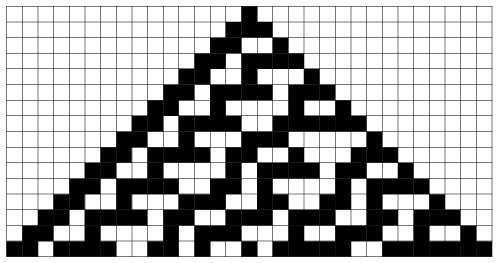
\includegraphics[width=70mm]{Imagenes/regla30en15.PNG}}
        \subfigure[Evolución del espacio $\mathcal{L}$ luego de 250 iteraciones]{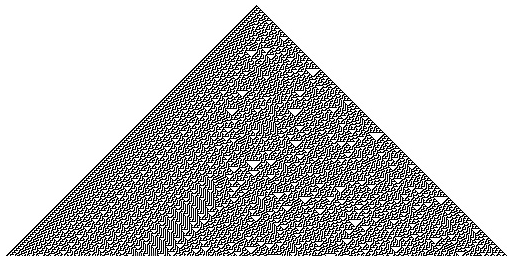
\includegraphics[width=70mm]{Imagenes/regla30en250.PNG}}
        \caption{Evoluciones al aplicar la regla 30 de Wolfram. Captura tomada de \cite{rule30}}
    \end{figure}
    
    %%%%%%%%%%%%%%%%%%%%%%%%%%%%%%%%%%%%%%%%%%%%%%%%%%%%%%%%%%%%%%%%%%%%%%%%%%%%%%%%%%%%%%%%%%%%
    % \newpage
    %%%%%%%%%%%%%%%%%%%%%%%%%%%%%%%%%%%%%%%%%%%%%%%%%%%%%%%%%%%%%%%%%%%%%%%%%%%%%%%%%%%%%%%%%%%%
    
    \item \textbf{Reglas totalísticas}
    
    A diferencia de las reglas determinísticas, las reglas totalísticas no establecen una correspondencia directa entre estados y combinaciones de vecindades, sino que en su lugar utilizan un componente probabilístico. Esto significa que dependiendo de la combinación, la célula sobre la que se aplica la regla puede tomar un estado de un subconjunto del conjunto de estados $\Sigma$. 
    
    Existe un subtipo de este tipo de reglas conocido como las reglas semi-totalísticas, en las que el subconjunto que se considera para la evolución de la célula sobre la que se aplica la regla, depende del estado de la misma célula. De ese modo, definimos una regla semi-totalística como:
    
    \begin{align*}
        \phi:\Sigma_x\times\overbrace{\Sigma\times\Sigma\times\cdots\times\Sigma}^{N}&\longrightarrow \left\{ \begin{array}{cc}
        \sigma_1 \subseteq \Sigma_x & \text{si el estado de }x\text{ es }s_1 \\
        \sigma_2 \subseteq \Sigma_x & \text{si el estado de }x\text{ es }s_2 \\
        \vdots & \vdots \\
        \sigma_k \subseteq \Sigma_x & \text{si el estado de }x\text{ es }s_k
        \end{array} \right. ,
    \end{align*}
    
    donde $k$ es la cantidad de posibles estados que puede tomar $x$.
\end{itemize}

A pesar de que las reglas determinísticas pueden generar resultados interesantes su implementación computacional no resulta muy cómoda, sobre todo si consideramos espacios de células de más de una dimensión. De acuerdo con \cite{alfons2010}, la cantidad de posibles combinaciones o reglas que se pueden definir si usáramos las del tipo determinista serían:

$$N_r=\#\Sigma^{\#\Sigma^N},$$

donde $\#\Sigma$ es la cantidad de estados en $\Sigma$ y $N$ es la cantidad de vecinos que se consideran en el sistema de vecindades. Por ejemplo, para el caso de la regla 30 la cantidad de reglas que se pueden definir es igual a $2^{2^2}=16$. Esto representa una complicación al trabajar con espacios de más de una dimensión por lo que para los propósitos del proyecto nos enfocaremos únicamente sobre las reglas totalísticas y para ser más específicos sobre las reglas semi-totalísticas, esto debido al contexto de nuestro proyecto.

Una vez aclarados todos los conceptos que abarcan los autómatas celulares podemos dar una definición formal de ellos:

\begin{definition}\label{def:automataCelular}
Un \textit{autómata celular} es una la tupla de la forma  $A=(\mathcal{L},\Sigma,\mathcal{N}(\mathcal{L}),\phi)$ con $\mathcal{N}(\mathcal{L})$ un sistema de vecindades sobre $\mathcal{L}$.
\end{definition}

En el siguiente capítulo nos enfocaremos en unificar los conceptos que vimos a lo largo de este capítulo, para luego definir las reglas de evolución que permitirán describir las interacciones entre células y la manera en la que una enfermedad las puede afectar.
\chapter{Modelos epidemiológicos en autómatas celulares}\label{cap:Modelos epidemiológicos en AC}

Pensemos por un momento en que si un individuo susceptible a una enfermedad tiene contacto con muchos infectados, puede enfermarse con mucha más facilidad que un individuo que tiene contacto con pocos infectados. Ahora bien ¿cuántas interacciones con infectados de todos las que puede llegar a tener una célula, son suficientes para generar una probabilidad de contagio más alta?, para responder a esto primero debemos determinar la naturaleza detrás de las posibles relaciones entre células y para esto haremos uso de herramientas como los sistemas fundamentales de vecindades.

Construiremos las reglas de evolución que definirán las dinámicas de cada modelo, partiendo de principios lógicos tomados directamente de los modelos clásicos descritos en el capítulo \ref{cap:Preliminares} y nociones de topología que permitan establecer las interacciones entre células.

A lo largo del capítulo también desarrollaremos una serie de ejemplos para explicar con mayor detalle el funcionamiento de cada regla y realizaremos una breve comparación con los resultados obtenidos de los modelos clásicos.

\section{Interacciones e impactos sociales}\label{sec:InteraccionesEImpactosSociales}
A diferencia del trabajo realizado en \cite{populationDensity} en el que cada celda representaba una región, consideraremos a cada división como un único individuo que será dotado de un conjunto de cualidades como estado de salud, edad, vecinos, etc. Estas cualidades vendrán dadas por las necesidades del modelo que estemos desarrollando, por ejemplo en los modelos clásicos no será necesario dotar de edades a las células, pero si tendremos que tener en cuenta sus vecindades y sus estados de salud.

Pensemos por un momento en las características que hay detrás de relación cercana entre individuos o células. Denotaremos la relación entre células con el símbolo $\thicksim$ y una vez dicho esto tenemos que:

\begin{itemize}
    \item Todas las células están en contacto con ellas mismas, por lo que para cada célula $x$ se cumple $x \thicksim x$.
    \item Si una célula estuviera en contacto con alguna otra entonces esa célula estaría en contacto con la primera, es decir, $x\thicksim y$ implica $y\thicksim x$.
    \item Si una célula interactúa con otras dos no implica necesariamente que estas interactúen entre sí, por lo que $x\thicksim y$ y $x\thicksim z$ no implican que $y\thicksim z$.
\end{itemize}

\begin{example}\label{ex:relacionesExBase}
Consideremos por ejemplo el conjunto $X=\{a,b,c\}$ y a la sub-colección $\mathcal{A}$ del ejemplo \ref{ex:exBase} dado por $\mathcal{A}=\{\emptyset,\{a\},\{b\}.\{a,b\},\{a,c\},\{a,b,c\}\}$. Entonces se obtienen las siguientes relaciones

$$\begin{array}{cccccc}
    a\thicksim a, & b\thicksim b, & a\thicksim b, & a\thicksim c & \text{, y} & b\thicksim c,
\end{array}$$

junto con sus relaciones simétricas equivalentes.
\end{example}

La noción de relación del ejemplo \ref{ex:relacionesExBase} de interacción entre células puede ir un poco más allá. Pensemos por un momento en el impacto que puede tener un comportamiento sobre la célula $b$ en la célula $a$, si bien estas dos celdas no interactúan entre sí, la relación que cada una de ellas tiene con las células $c$ y $d$ puede tener un impacto sobre la otra. Con lo cual definimos la siguiente relación de interacción:

\begin{definition}\label{def:gradoDeImpacto}
Definimos el \textit{grado de impacto} entre dos puntos $a$ y $b$ como la menor cantidad de interacciones necesaria para llegar de $a$ a $b$. Para reconocer el grado de impacto entre dos puntos usaremos la notación $a\thicksim_n b$ donde $n\in\mathbb{N}$ denota la menor cantidad de interacciones entre $a$ y $b$.
\end{definition}

Si retomamos el ejemplo \ref{ex:relacionesExBase} podremos identificar los siguientes grados de impacto:

$$\begin{array}{ccccccc}
    a\thicksim_0 a, & b\thicksim_0 b, & a\thicksim_1 c, & a\thicksim_1 b, &
    b\thicksim_1 a, & b\thicksim_2 c, & c\thicksim_0 a
\end{array}$$
\begin{figure}[h]\label{fig:gradoImpacto}
  \centering
    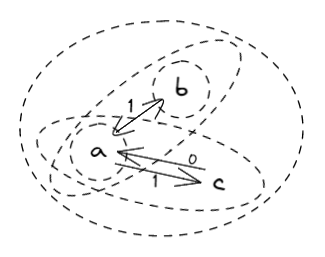
\includegraphics[width=0.3\textwidth]{Imagenes/grados_de_impacto.PNG}
  \caption{Grados de impacto para el espacio $X$ con la topología $\mathcal{A}$.}
\end{figure}

De la definición \ref{def:gradoDeImpacto} podemos deducir el siguiente resultado:

\begin{teorema}\label{teo:gradeosDeImpactoImplicaSFV}
Los grados de impacto de una célula $x$ definen un sistema fundamental de vecindades.
\end{teorema}
\begin{proof}
Sea $x\in\mathcal{L}$ y $\mathcal{V}(x)$ una familia de vecindades de $x$. Defina el conjunto $A_0$ como el conjunto de puntos con grado de impacto con $x$ es igual a cero y de manera recursiva a los conjuntos $A_k$, cuyos elementos tienen grado de impacto con $x$ sea igual o menor a $k$. Claramente $A_i\subseteq A_j$ para $0\leq i\leq j$ y de ese modo $A_i\in\mathcal{V}(x)$ para $i=0,1,\cdots,n$.

Veamos ahora que el conjunto $A_0$ es la vecindad mínimal de $x$. Considere $y\in U_x$, en particular $y\in\bigcap\mathcal{V}(x)$ por la definición de 2.4.14. Si el grado de impacto de $y$ con $x$ es mayor a cero por la definición 3.1.2 podemos afirmar que existe $z\in\mathcal{L}$ tal que $z\thicksim x$, $z\thicksim y$ y $x\not\thicksim y$ y de ese modo $x$ e $y$ son puntos separables. Esto es una contradicción por el hecho de que $y\in \bigcap \mathcal{V}(x)$ y por lo tanto $y\thicksim_0 x$, es decir $y\in A_0$.

Considere $y\in A_0$ y por la definición de grado de impacto cero, afirmamos que los puntos $x$ e $y$ no son separables por lo que $y\in\mathcal{V}(x)$ y con esto concluimos la prueba.
\end{proof}

A continuación mostraremos algunas de las propiedades del conjunto $\mathcal{A}$ definido en la demostración anterior:

\begin{proposicion}\label{pro:propiedadesSistemasDeVecindadesEncajadas}
Sea $x\in\mathcal{L}$ una célula y sea $\mathcal{A}$ la familia de conjuntos encajados definidos por el grado de impacto con $x$. Se cumplen las siguientes propiedades:
\begin{enumerate}
    \item El conjunto $\mathcal{A}$ posee elemento mínima igual a $A_0$,
    \item $\mathcal{A}$ es un conjunto ordenado finito con el orden de la contenencia, y
    \item $\mathcal{L}$ es un espacio uno-numerable.
\end{enumerate}
\end{proposicion}
\begin{proof}
Cada numeral se deduce directamente de las definiciones \ref{def:vecindadMinimal}, \ref{def:conjuntoPreordenadoFinito}, \ref{def:espacio1Numerable} y el teorema \ref{teo:gradeosDeImpactoImplicaSFV}.
\end{proof}

Algo que debemos tener en cuenta es que el grado de impacto por si solo no nos proporciona una medida del impacto que tienen los cambios de estado de células "lejanas" (o de grado de impacto mayor a cero). Estas medidas de impacto se entenderán como la probabilidad de que un cambio de estado afecte a la célula con la que estamos realizando la comparación, de ese modo las tasas de impacto serán valores entre 0 y 1 que pueden venir dados por cualquier tipo de función que tenga como dominio al conjunto de grados de impacto.

\begin{example}
Consideremos las siguientes matrices que describen los grados de impacto en tres distintos sistemas fundamentales de vecindades para la célula en la posición 2,2:

\begin{figure}[h]\label{fig:gradoImpacto}
  \centering
    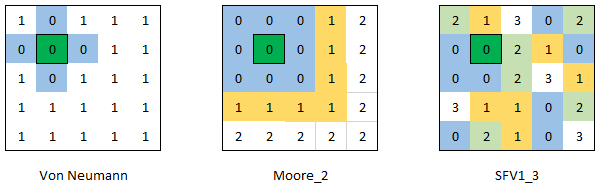
\includegraphics[width=0.7\textwidth]{Imagenes/ex315.PNG}
  \caption{Grados de impacto en diferentes sistemas de vecindades.}
\end{figure}

En la figura \ref{fig:gradoImpacto} podemos ver que debido a la manera en la que implementamos nuestro espacio de células, es posible representar los grados de impacto de cada una con una célula particular en un arreglo matricial, al igual que los estados de cada célula como se vio en el capítulo dos.

La asignación entre grados y tasas de impacto puede escogerse de cualquier manera dependiendo del contexto y la enfermedad que esté modelando. Para los efectos del ejemplo consideraremos las siguientes matrices de tasas de impacto (figura (\ref{fig:tasaImpacto})):

\begin{figure}[h]\label{fig:tasaImpacto}
  \centering
    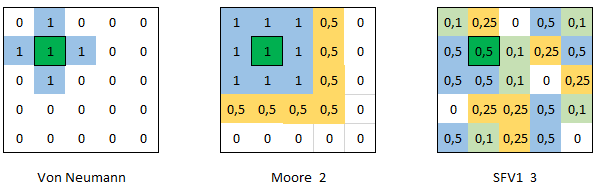
\includegraphics[width=0.7\textwidth]{Imagenes/ex3152.PNG}
  \caption{Tasas de impacto en diferentes sistemas de vecindades.}
\end{figure}
\end{example}

Una vez establecidos los conceptos de topología implementados para nuestro espacio $\mathcal{L}$ y sus sistemas fundamentales de vecindades podemos definir cada una de las reglas que implementaremos para cada modelo epidemiológico.

\section{Reglas de evolución}\label{sec:ReglasDeEvolución}

Partiremos de una abstracción sobre la naturaleza de los modelos epidemiológicos definidos en el capítulo \ref{cap:Preliminares}, esto nos permitirá definir de manera intuitiva las reglas de evolución de nuestros modelos en autómatas celulares.

Antes de comenzar a definir nuestras reglas de evolución definiremos las siguientes notaciones:
\begin{itemize}
    \item El estado de la célula $x$ en un momento $t$ se denotará como $\pi^t(x)$.
    \item La cantidad de individuos con grado de impacto $g$ y estado $K$ de una célula $x$ en un momento $t$ será representado como $\sigma_{g,K}^t(x)$.
    \item Para representar a la cantidad de individuos con un grado de impacto $g$ usaremos el símbolo $\Delta_g$. 
    \item Usaremos los símbolos $\mathcal{S}^t,\mathcal{I}^t,\mathcal{R}^t$ y $\mathcal{D}^t$ para denotar a los conjuntos de células susceptibles, infectadas, recuperadas y muertas respectivamente en el espacio $\mathcal{L}$ en el tiempo $t$. De manera formal
    $$\mathcal{S}^t=\{x\in\mathcal{L}:\pi^t(x)=S\},$$
    y de manera análoga se definen los conjuntos $\mathcal{I}^t,\mathcal{R}^t$ y $\mathcal{D}^t$. Note que $$\mathcal{S}^t\cup\mathcal{I}^t\cup\mathcal{R}^t\cup\mathcal{D}^t=\mathcal{L}\text{ para todo tiempo }t.$$
\end{itemize}

\subsection{Modelos SIS y SIR simples}\label{sub:SISySIRSimples}

Recordemos que para las tasas de infección $\beta$ y de recuperación $\alpha$ los modelos SIS y SIR nos afirman que para $\mathcal{R}_0=\frac{\beta}{\alpha}>1$ la enfermedad será endémica. Trataremos de replicar inicialmente esté comportamiento de manera local sobre una célula analizando los siguientes puntos:

\begin{itemize}
    \item La probabilidad de que un individuo susceptible se enferme depende no solo de la enfermedad, sino que además depende de la cantidad de individuos infectados que tenga en su sistema de vecindades locales, atada a las tasas de impacto que definimos en la sección anterior. 
    \item Como vimos en el capítulo \ref{cap:Preliminares} la recuperación de los individuos infectados no se ve afectada por la cantidad de contactos con otras células y en lugar de eso depende completamente de la tasa de recuperación $\alpha$, la cual en nuestro caso entenderemos como la proporción de individuos infectados que se recuperan de la enfermedad.
    \item Para el estado de inmunidad en el modelo SIR, supondremos que los individuos que posean este estado se mantendrán inmunes. Esto quiere decir que la transformación para individuos recuperados será constante.
\end{itemize}

Dado que los modelos SIS y SIR comparten el paso del estado S al estado I definiremos primero la regla de evolución para un modelo SI:

\begin{definition}\label{def:reglaSI}
Para una célula $x$ en un espacio $\mathcal{L}$ definimos la regla SI como:
\begin{equation}
    \phi_{SI}^t(x)=\left\{\begin{array}{ll}
        S & \text{si }\pi^t(x)=S\text{, }\sum_g{\sigma_{g,I}^t(x)\cdot P(g)}\leq \sum_g{\sigma_{g,S}^t(x)\cdot P(g)}\text{ y }\rho\geq i(t),\\
        I & \text{si }\pi^t(x)\in\{S,I\}\text{,} \\
        \pi^t(x) & \text{en otro caso,}
    \end{array}\right.
\end{equation}
con $\rho\in\mathcal{U}_{[0,1]}$, $P(g)$ la tasa de impacto del grado $g$ e
\begin{equation}
    i(t) = \frac{\beta}{\alpha}\sum_g{\frac{\sigma_{g,I}^t(x)}{\Delta_g}}\cdot P(g).
\end{equation}
\end{definition}

\begin{example}\label{ex:SIenAutómatasCelulares}
En la figura \ref{fig:configuraciónInicialEspacio25Celulas} podemos encontrar la configuración de estados para un sistema de 25 células: en las tres del lado derecho encontramos la disposición de grados de impacto para las tres células marcadas en color verde (primera imagen), donde SFV es una abreviación de Sistema Fundamental de Vecindades.

%%%%%%%%%%%%%%%%%%%%%%%%%%%%%%%%%%%%%%%%%%%%%%%%%%%%%%%%%%%%%%%%%%%%%%%%%%%%%%%%%%%%%%%%%%%%%%%%%
\newpage
%%%%%%%%%%%%%%%%%%%%%%%%%%%%%%%%%%%%%%%%%%%%%%%%%%%%%%%%%%%%%%%%%%%%%%%%%%%%%%%%%%%%%%%%%%%%%%%%%

\begin{figure}[h]\label{fig:configuraciónInicialEspacio25Celulas}
  \centering
    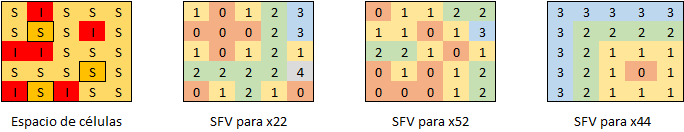
\includegraphics[width=0.9\textwidth]{Imagenes/cellSpace.PNG}
    \caption{Configuración inicial de estados y sistemas fundamentales de vecindades}
\end{figure}

Consideraremos las siguientes tasas de impacto:

\begin{table}[h]
\begin{center}
\begin{tabular}{| c | c |}
\hline
Grados & Tasas \\ \hline
0 & 0.5 \\
1 & 0.3\\
2 & 0.25\\
3 & 0.1\\ 
4 & 0.05\\ \hline
\end{tabular}
\caption{Relación entre tasas y grados de impacto.}
\end{center}
\end{table}

A continuación calcularemos las magnitudes ponderadas de individuos susceptibles e infectados y la probabilidad de infectarse para cada una de las tres células:

\begin{itemize}
    \item Célula $x_{2,2}$:
    \begin{align*}
    \begin{array}{l}
        \sum_g\sigma_{g,S}^0(x_{2,2})\cdot P(g) = 4\cdot0.5+6\cdot0.3+6\cdot0.25+2\cdot0.1+1\cdot0.05 = 5.55 \\
        \sum_g\sigma_{g,I}^0(x_{2,2})\cdot P(g) = 3\cdot0.5+1\cdot0.3+2\cdot0.25+0\cdot0.1+0\cdot0.05 = 2.3\\
        i_{2,2}(0) = \frac{\beta}{\alpha}\cdot\left(\frac{3\cdot0.5}{7}+\frac{1\cdot0.3}{7}+\frac{2\cdot0.25}{8}+\frac{0\cdot0.1}{2}+\frac{0\cdot0.05}{1}\right)=\frac{179}{560}\cdot\frac{\beta}{\alpha}
    \end{array}
    \end{align*}
    \item Célula $x_{5,2}$:
    \begin{align*}
    \begin{array}{l}
        \sum_g\sigma_{g,S}^0(x_{5,2})\cdot P(g) = 6\cdot0.5+8\cdot0.3+4\cdot0.25+1\cdot0.1+0\cdot0.05 = 6.5 \\
        \sum_g\sigma_{g,I}^0(x_{5,2})\cdot P(g) = 2\cdot0.5+2\cdot0.3+2\cdot0.25+0\cdot0.1+0\cdot0.05 = 2.1\\
        i_{5,2}(0) = \frac{\beta}{\alpha}\cdot\left(\frac{2\cdot0.5}{8}+\frac{2\cdot0.3}{10}+\frac{2\cdot0.25}{6}+\frac{0\cdot0.1}{1}\right)=\frac{161}{600}\cdot\frac{\beta}{\alpha}
    \end{array}
    \end{align*}
    \item Célula $x_{4,4}$:
    \begin{align*}
    \begin{array}{l}
        \sum_g\sigma_{g,S}^0(x_{4,4})\cdot P(g) = 1\cdot0.5+7\cdot0.3+5\cdot0.25+6\cdot0.1+0\cdot0.05 = 4.45 \\
        \sum_g\sigma_{g,I}^0(x_{4,4})\cdot P(g) = 0\cdot0.5+1\cdot0.3+2\cdot0.25+3\cdot0.1+0\cdot0.05 = 1.1\\
        i_{4,4}(0) = \frac{\beta}{\alpha}\cdot\left(\frac{0\cdot0.5}{1}+\frac{1\cdot0.3}{8}+\frac{2\cdot0.25}{7}+\frac{3\cdot0.1}{9}\right)=\frac{239}{1680}\cdot\frac{\beta}{\alpha}
    \end{array}
    \end{align*}
\end{itemize}

Podemos apreciar que las magnitudes ponderadas tanto de individuos susceptibles como de infectados son diferentes para cada célula son diferentes. Es implica que las probabilidades de contagiarse de la enfermedad están directamente relacionados con la manera en la que las células interactúan con las demás.\la

En este caso las tres células pueden o no contagiarse de la enfermedad si aplicamos la regla $\phi_{SI}^t(x)$. Supongamos que la enfermedad cuenta con una tasa de infección $\beta=0.5$ y una tasa $\alpha=0.2$, de ese modo las probabilidades de adquirir la enfermedad son:
$$\begin{array}{ccccc}
    i_{2,2}(0)=0.8, & i_{5,2}(0)=0.675. & \text{e} & i_{4,4}(0)=0.35.
\end{array}$$
Podemos observar que la célula $x_{4,4}$ tiene una probabilidad menor de adquirir la enfermedad, esto se debe a que según el sistema de vecindades escogido la célula se encuentra más alejada de los infectados que las células $x_{2,2}$ y $x_{5,2}$.
\end{example}

La definición \ref{def:reglaSI} nos permite definir de manera natural a las reglas de evolución para los modelos SIS y SIR en autómatas celulares:

\begin{definition}\label{def:reglasSISySIR}
Dada una célula $x$ en un conjunto $\mathcal{L}$ definimos respectivamente las reglas de evolución para los modelos SIS y SIR respectivamente como:
\begin{equation}
    \phi_{SIS}^t(x)=\left\{\begin{array}{ll}
        \phi_{SI}^t(x) & \text{si }\pi^t(x) = S,\\
        I & \text{si }\pi^t(x)=I\text{ y }\rho>\alpha,\\
        S & \text{si }\pi^t(x)=I\text{ y }\rho\leq\alpha.
    \end{array}\right.
\end{equation}

\begin{equation}
    \phi_{SIR}^t(x)=\left\{\begin{array}{ll}
        \phi_{SI}^t(x) & \text{si }\pi^t(x) = S,\\
        I & \text{si }\pi^t(x)=I\text{ y }\rho>\alpha,\\
        R & \text{si }\pi^t(x)=I\text{ y }\rho\leq\alpha, y \\
        R & \text{si }\pi^t(x)=R,
    \end{array}\right.
\end{equation}
donde $\rho\in\mathcal{U}_{[0,1]}$.
\end{definition}

\textbf{Observación:} Dado que las reglas $\phi_{SIS}^t(x)$ y $\phi_{SIR}^t(x)$ actúan como una composición de funciones para el estado $S$, podemos establecer el orden de aplicación de reglas de adentro hacia afuera, esto significa que computacionalmente tendremos que aplicar primero la regla $\phi_{SI}^t(x)$ y luego las probabilidades para la recuperación de los individuos.

\begin{example}\label{ex:SISySIRenAutomatasCelulares}
Consideremos la configuración de estados del ejemplo anterior junto con las tasas de infección y recuperación $\beta=0.5$ y $\alpha=0.2$ respectivamente. De acuerdo con la definición \ref{def:reglaSI} y la observación anterior, si aplicamos las reglas $\phi_{SIS}^t(x)$ y $\phi_{SIR}^t(x)$ podremos observar un comportamiento similar a los siguientes:

%%%%%%%%%%%%%%%%%%%%%%%%%%%%%%%%%%%%%%%%%%%%%%%%%%%%%%%%%%%%%%%%%%%%%%%%%%%%%%%%%%%%%%%%%%%%%%%%%
\newpage
%%%%%%%%%%%%%%%%%%%%%%%%%%%%%%%%%%%%%%%%%%%%%%%%%%%%%%%%%%%%%%%%%%%%%%%%%%%%%%%%%%%%%%%%%%%%%%%%%

\begin{figure}[h]
  \centering
    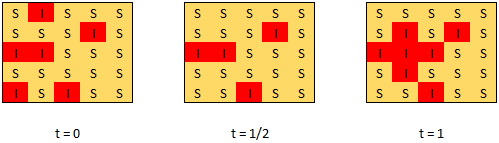
\includegraphics[width=0.7\textwidth]{Imagenes/sisAplication.PNG}
    \caption{Aplicación de la regla $\phi_{SIS}^t(x)$}
\end{figure}

\begin{figure}[h]
  \centering
    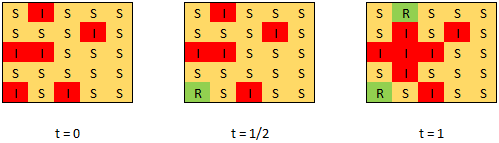
\includegraphics[width=0.7\textwidth]{Imagenes/sirAplication.PNG}
    \caption{Aplicación de la regla $\phi_{SIR}^t(x)$}
\end{figure}

Como se puede observar en la aplicación de ambas reglas existe una unidad temporal intermedia en la que se aplica la regla $\phi_{SI}^t(x)$ para luego aplicar la regla sobre el estado $I$. En el caso del modelo SIS vemos que las células pasan al estado $S$ de acuerdo con las reglas del modelo clásico y de manera similar con el modelo SIR.
\end{example}

\textbf{Observación:} Es importante recordar que el paso del estado $I$ al estado $S$ o al $R$ no depende del sistema de vecindades, ya que se asume que no es necesario el contacto con células no infectadas para que una que se encuentra enferma se recupere.

\begin{example}\label{ex:SISySIRclásicovsModeloEnAC}
Consideremos dos espacios de 900 células en donde una misma enfermedad actúa de manera diferente. Mientras que en el primer espacio los individuos no generan inmunidad tras recuperarse de la enfermedad, en el segundo espacio si y durante un tiempo indefinido.

Las tasas de infección y de recuperación de la enfermedad son $\beta=0.5$ y $\alpha=0.2$, lo que implica que la enfermedad será endémica, pues $\mathcal{R}_0=\frac{\beta}{\alpha}=2.5>1$. Asumiremos que el brote de infectados inicial se ubicó en la zona central de ambos espacios y que las interacciones entre células se describen a partir del sistema de vecindades generado por las vecindades de Moore. La evolución de la enfermedad en ambos espacios se puede apreciar en las figuras (\ref{fig:sisEn30}) y (\ref{fig:sirEn30}).

%%%%%%%%%%%%%%%%%%%%%%%%%%%%%%%%%%%%%%%%%%%%%%%%%%%%%%%%%%%%%%%%%%%%%%%%%%%%%%%%%%%%%%%%%%%%%%%%%
\newpage
%%%%%%%%%%%%%%%%%%%%%%%%%%%%%%%%%%%%%%%%%%%%%%%%%%%%%%%%%%%%%%%%%%%%%%%%%%%%%%%%%%%%%%%%%%%%%%%%%

\begin{figure}[h]\label{fig:sisEn30}
  \centering
    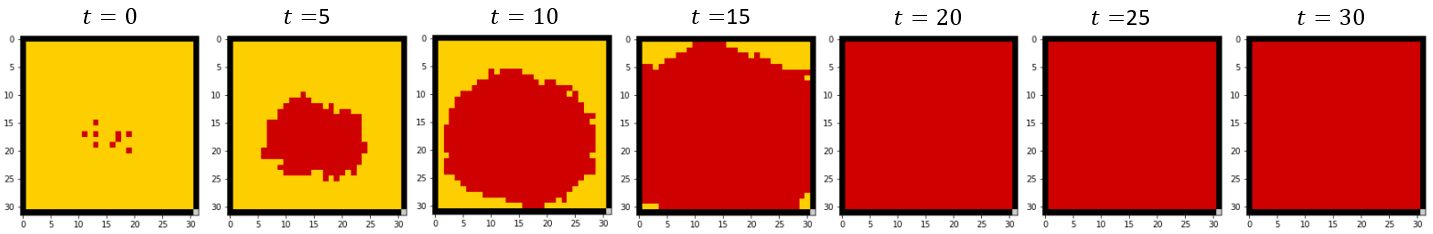
\includegraphics[width=0.93\textwidth]{Imagenes/sisEn30.PNG}
    \caption{Evolución de la enfermedad en 30 días (modelo SIS).}
\end{figure}
\begin{figure}[h]\label{fig:sirEn30}
  \centering
    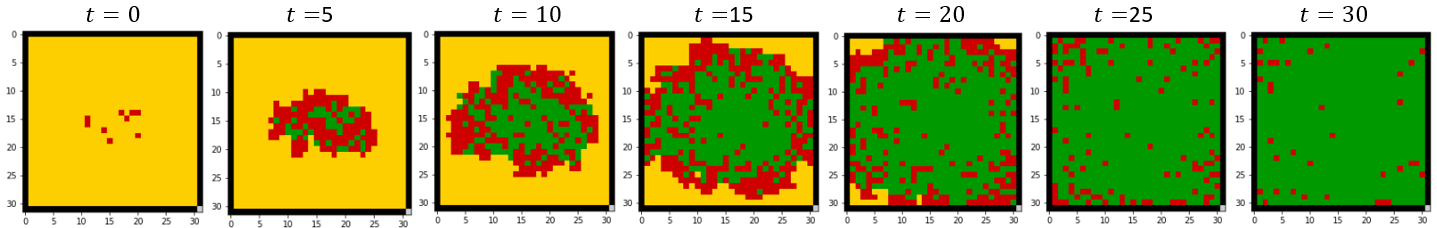
\includegraphics[width=0.93\textwidth]{Imagenes/sirEn30.PNG}
    \caption{Evolución de la enfermedad en 30 días (modelo SIR).}
\end{figure}

A continuación podremos visualizar las soluciones obtenidas al analizar el mismo escenario con los modelos clásicos (izquierda) y las generadas por nuestras reglas de evolución $\phi_{SIS}^t(x)$ y $\phi_{SIR}^t(x)$ (derecha):

\begin{figure}[h]\label{fig:sirEn30}
  \centering
    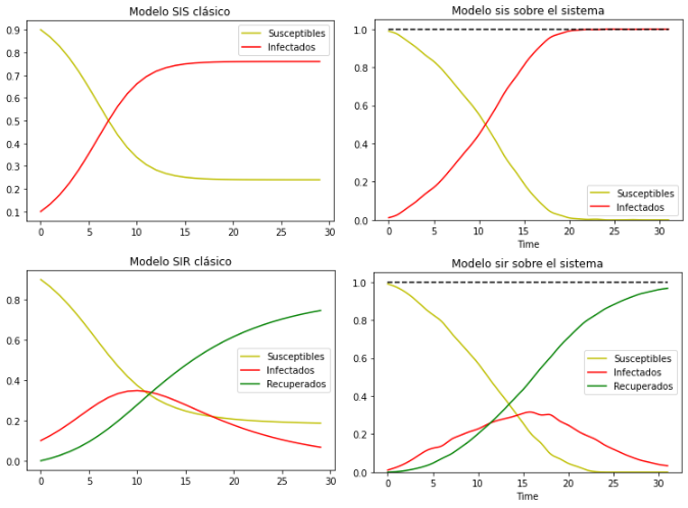
\includegraphics[width=0.6\textwidth]{Imagenes/solucionesSISySIR1.PNG}
    \caption{Evolución de la enfermedad en 30 días (modelos clásicos vs reglas de evolución).}
\end{figure}
\end{example}

\subsection{Modelos con natalidad y mortalidad}\label{sub:NatalidadyMortalidad}
Partiendo del principio de que los análisis desarrollados en nuestra investigación tengan una mayor aplicabilidad en el ámbito epidemiológico decidimos separarnos un poco de los modelos clásicos, ya que en estos se supone que las tasas de natalidad y mortalidad son iguales y esto no necesariamente se cumple en el mundo real.

La segunda característica que tendremos en mente para definir nuestra regla de evolución parte de hipótesis de que los individuos en un sistema tienen una probabilidad de fallecer por causas ajenas a la enfermedad que depende de la edad del mismo individuo.

Para implementar la noción de edad de una célula inicialmente tendremos que modificar el dominio de nuestra regla de evolución. Para estos modelos debemos tener en cuenta el estado de la célula central junto con su edad y el estado de sus vecinos, de modo que 
$$Dom(\phi_\mu)=\Sigma_x\times K\times\overbrace{\Sigma\times\cdots\times\Sigma}^N\text{, con }K=\{1,2,\cdots,100\},$$
si suponemos que la edad de la célula $x$ puede ir de 1 a 100 unidades temporales (semanas, meses, años, etc.).

Otra característica que podemos implementar en nuestro modelo es la del envejecimiento de las células, esto con el objetivo de analizar el impacto de una enfermedad sobre los individuos de un sistema en diferentes etapas de su "vida". La manera en la que abordaremos esta idea será con el siguiente ajuste en el rango de nuestra regla
$$Ran(\phi_\mu)=\Sigma_x\times K.$$
Dado que estamos trabajando sobre poblaciones de tamaño constante la manera en la que interpretaremos el nacimiento de una célula será con la ocupación del espacio que deja una que muere. Para esto identificaremos a los espacios que dejan las células que mueren con el estado $D$ y una edad cero, esto nos permitirá separar a los espacios que pueden ocuparse y los que no de células que interactúen con sus vecinos. Al igual que en los modelos descritos en el capítulo 1 asumiremos que los individuos que "nacen" son susceptibles a la enfermedad.

Teniendo estas ideas en mente podemos definir la regla de evolución para un modelo epidemiológico $M$ de la siguiente manera:

\begin{definition}\label{def:reglaNatalidadyMortalidad}
Sea $x$ una célula en un conjunto $\mathcal{L}$, $M$ un modelo epidemiológico y $T$ una unidad temporal (días, meses, años, etc.). Definimos la regla de evolución con nacimientos y muertes para $M$ como:
\begin{equation}
    \mu_{M,T}^t(x)=\left\{\begin{array}{ll}
        D,0 & \text{si }t\not\equiv 0 \text{ (modulo }T\text{), }\pi^t(x)\in\{S,I,R\}\text{ y }\rho\leq\omega_k, \\
        D,0 & \text{si }\pi^t(x)=D\text{ y }\rho>b,\\
        S,1 & \text{si }\pi^t(x)=D\text{ y }\rho\leq b,\\
        \phi_M^t(x),E^t(x) & \text{si }t\not\equiv 0 \text{ (modulo }T),\\
        \phi_M^t(x),E^t(x)+1 & \text{si }t\equiv 0 \text{ (modulo }T),
    \end{array}\right.
\end{equation}
donde $\omega_k$ es la probabilidad de morir por causas ajenas a la enfermedad para las edades en la partición k-ésima del intervalo $[0,100]$, $b$ es la tasa de natalidad, $\phi_M^t$ es la regla de evolución del modelo epidemiológico, $E^t(x)$ denota la edad de la célula $x$ en el momento $t$ y $\rho\in\mathcal{U}_{[0,1]}$.
\end{definition}

\begin{example}\label{ex:natalidadyMortalidad}
Consideremos una probabilidad de nacimiento (u ocupación de espacios disponibles) $b=0.02$ y una unidad temporal $T=2$ sobre la siguiente configuración de estados en un espacio de células junto con las probabilidades de muerte por grupo de edad: 

\begin{figure}[h]\label{ex:configuraciónInicialNatalidadyMortalidad}
  \centering
    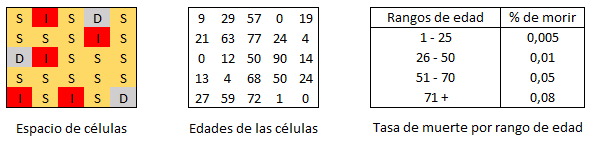
\includegraphics[width=0.8\textwidth]{Imagenes/conInicialMNM.PNG}
    \caption{Configuración inicial para el espacio de células y tasas de muerte por edad.}
\end{figure}

Dado que las células que posean una edad igual a cero no podrán interactuar con las demás debido a su misma definición, podemos afirmar que existe una dependencia entre el estado de la célula y su edad por lo que antes de aplicar la regla de evolución del modelo epidemiológico (SIS o SIR), aplicaremos la regla para los cambios sobre las edades de la célula de acuerdo con la definición \ref{def:reglaNatalidadyMortalidad}.

\begin{figure}[h]\label{ex:aplicaciónReglaNatalidadyMortalidad}
  \centering
    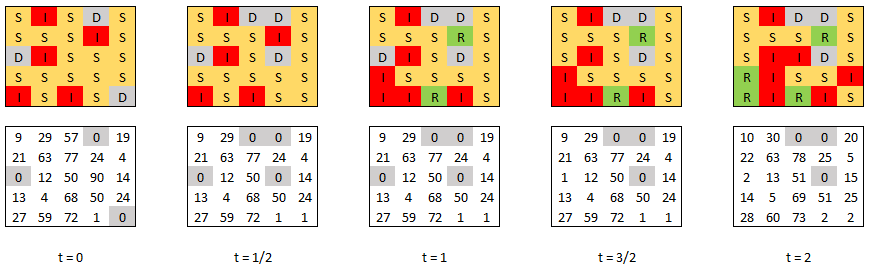
\includegraphics[width=1\textwidth]{Imagenes/natalidadMortalidad.PNG}
    \caption{Aplicación de la regla $\mu_{SIR,2}^t(x)$}
\end{figure}

En la figura \ref{ex:aplicaciónReglaNatalidadyMortalidad} podemos observar la aplicación del modelo SIR con natalidad y mortalidad en donde en particular en los tiempos $t=1/2$ y $t=3/2$ mueren y nacen nuevas células de acuerdo con las probabilidades de muerte por rango de edad y tasa de nacimiento establecidas. Por otra parte y de acuerdo con la definición del parámetro $T$, todas las células cumplen un ciclo (que puede entenderse como un año) cuando $t\equiv0$ (Módulo $T$).
\end{example}

\begin{example}\label{ex:sisClásicovsModeloEnAC}
Consideremos ahora una enfermedad que actúa sobre un espacio de 100 células y que posee tasas de infección de recuperación $\beta=0.05$ y $\beta=0.2$. Para comparar los resultados con el modelo clásico asumiremos que las tasas de natalidad y mortalidad son iguales a $\mu=\frac{1}{75\cdot6}$ (esperanza de vida de 75 años y $T=6$, es decir, las medidas se toman cada 2 meses). En particular podemos observar que la enfermedad no será endémica, pues $\mathcal{R}_0=\frac{\beta}{\alpha+\mu}\approx0.25<1$.

\begin{figure}[h]\label{ex:aplicaciónReglaNatalidadyMortalidad}
  \centering
    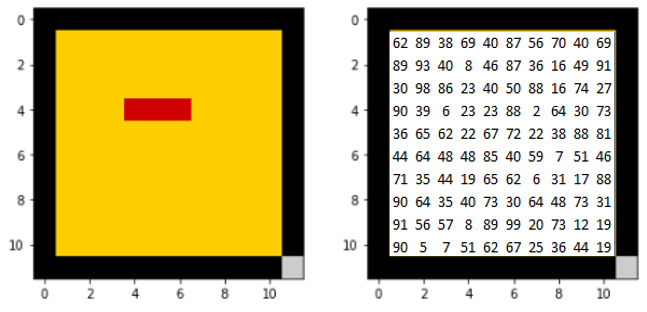
\includegraphics[width=0.6\textwidth]{Imagenes/sistemaYEdades.PNG}
    \caption{Configuración inicial de estados y de edades}
\end{figure}

A continuación ejecutaremos 40 veces la regla de evolución $\mu_{SIS,6}^t(x)$ y comparemos los resultados con los generados por el modelo clásico (figura (\ref{ex:aplicaciónReglaNatalidadyMortalidad})). Podemos observar que en ambos casos la población de infectados tiende a cero y que la cantidad de espacios libres (o células muertas) no crece demasiado, esto se debe a la baja probabilidad de muerte de nuestro espacio de células.

\begin{figure}[h]\label{ex:aplicaciónReglaNatalidadyMortalidad}
  \centering
    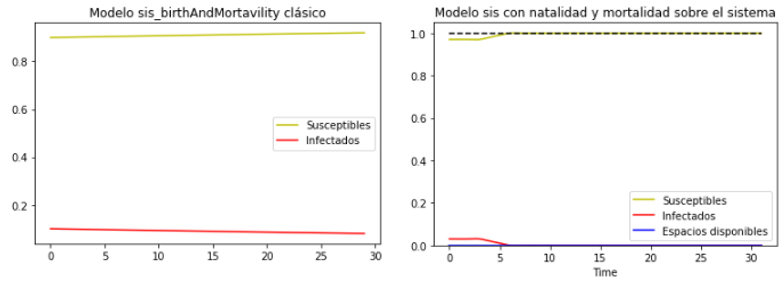
\includegraphics[width=0.75\textwidth]{Imagenes/solucionesNatalidadYMortalidad.PNG}
    \caption{Evolución de la enfermedad en 30 bimestres (modelo clásico y regla $\mu_{SIS,6}^t(x)$)}
\end{figure}
\end{example}

\subsection{Modelos con muerte por enfermedad}\label{sub:MuertePorEnfermedad}
En esta sección nos enfocaremos en definir la versión más general de los modelos epidemiológicos clásicos en ecuaciones diferenciales definidas en el capítulo 1. La muerte por enfermedad afectará únicamente a las células que posean la enfermedad y, buscando una mayor aplicabilidad sobre eventos más realistas asumiremos que la enfermedad puede tener un mayor impacto mortal sobre algunas edades. 

Al igual que en la sección anterior, realizaremos una partición sobre el intervalo $[0,100]$ y definiremos una probabilidad $\theta_k$ que indique la probabilidad de morir a causa de la enfermedad en la k-ésima partición. De manera formal:

\begin{definition}\label{def:reglaMuertePorEnfermedad}
Sea $x$ una célula en un conjunto $\mathcal{L}$, $M$ un modelo epidemiológico y $T$ una unidad temporal (días, meses, años, etc.). Definimos la regla de evolución con muerte por enfermedad para $M$ como:
\begin{equation}
    \theta_{M,T}^t(x)=\left\{\begin{array}{ll}
        D,0 & \text{si }\pi^t(x)=I\text{ y }\rho\leq\theta_k, \\
        \mu_{M,T}^t(x) & \text{en otro caso.}
    \end{array}\right.
\end{equation}
Donde $\theta_k$ es la probabilidad de morir por la enfermedad para los individuos con una edad en el intervalo k-ésimo de la partición del intervalo $[0,100]$, $\mu_{M,T}^t$ es la regla de evolución para modelos con nacimientos y muertes y $\rho\in\mathcal{U}_{[0,1]}$.
\end{definition}

\begin{example}
Partiremos del mismo escenario considerado en el ejemplo \ref{ex:natalidadyMortalidad} con las siguientes probabilidades de muerte por grupo de edad:

\begin{figure}[h]
  \centering
    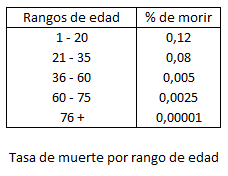
\includegraphics[width=0.3\textwidth]{Imagenes/muertePorEnfermedad.PNG}
\end{figure}

Al igual que en el ejemplo \ref{ex:natalidadyMortalidad}, la aplicación de la regla de evolución se realizará en dos fases: la primera fase corresponderá a los nacimientos, muertes por causas naturales, cambios en las edades de las células y la aplicación de las tasas de muerte causada por enfermedad por grupo de edad sobre los infectados y seguido de esto, se aplicará el modelo epidemiológico que corresponde a la segunda fase de nuestra regla de evolución.

\begin{figure}[h]
  \centering
    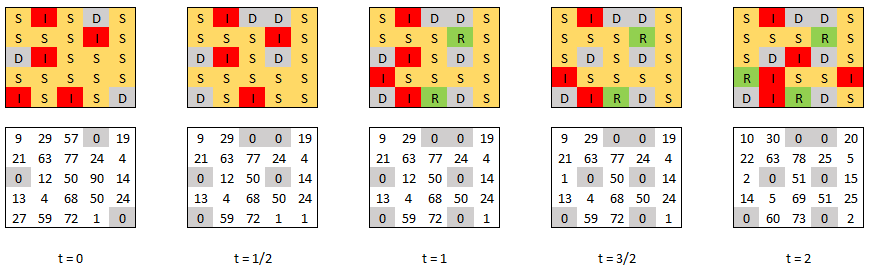
\includegraphics[width=1\textwidth]{Imagenes/muertePorEnfermedadEvo.PNG}
    \caption{Aplicación de la regla $\theta_{SIR,2}^t(x)$}
\end{figure}
\end{example}

\begin{example}\label{ex:muertePorEnfermedadClásicovsModeloEnAC}
Partiremos de la misma configuración de edades sobre un sistema de 100 células y las mismas tasas de natalidad y mortalidad consideradas en el ejemplo \ref{ex:aplicaciónReglaNatalidadyMortalidad}. Tomaremos las vecindades de Von Neumann para describir sus interacciones; en cuanto a la enfermedad, supondremos una tasa de infección $\beta=0.5$, una de recuperación $\alpha=0.2$ y una probabilidad de muerte causada por la misma enfermedad de $\theta=0.4$ (tomamos este valor con el objetivo de comparar los resultados con el modelo clásico).

\begin{figure}[h]\label{fig:muertePorEnfermedad10Veces}
  \centering
    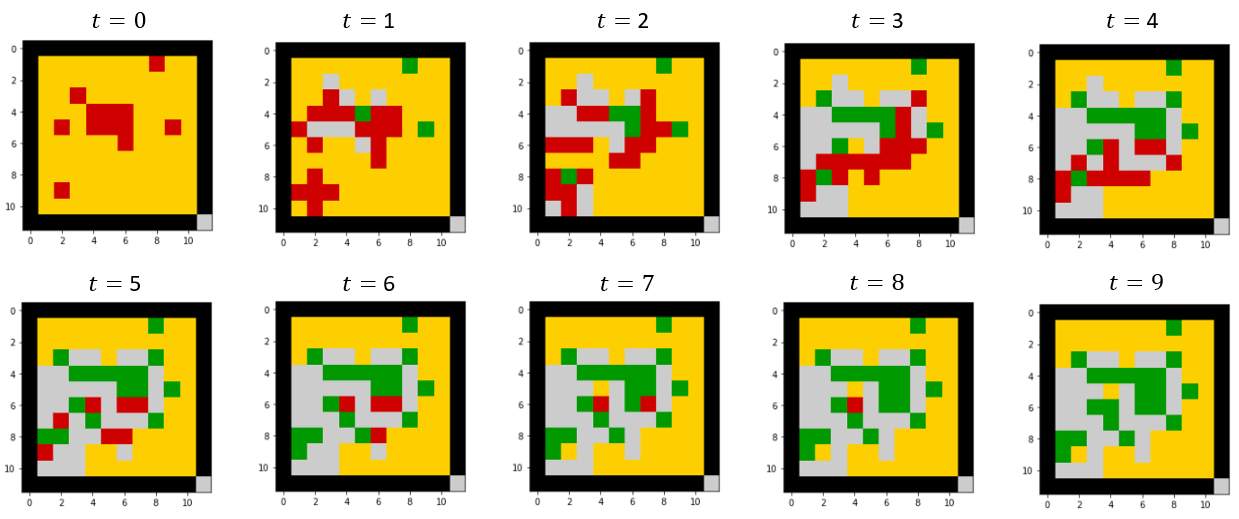
\includegraphics[width=1\textwidth]{Imagenes/evolucionesMuertePorEnfermedad.PNG}
    \caption{Aplicación de la regla $\theta_{SIR,6}^t(x)$ en 10 iteraciones}
\end{figure}

En la figura (\ref{fig:muertePorEnfermedad10Veces}) podemos observar que hay un incremento bastante pronunciado desde la segunda iteración hasta la quinta debido a la alta mortalidad de la enfermedad.

Una de las ventajas que ofrece nuestra librería es la de aplicar la regla de evolución varias veces y visualizar el comportamiento promedio de la enfermedad. A continuación aplicaremos la regla $\theta_{SIR,6}^t(x)$ 10 veces y compararemos los resultados con el modelo clásico:

\begin{figure}[h]\label{fig:muertePorEnfermedad10Veces}
  \centering
    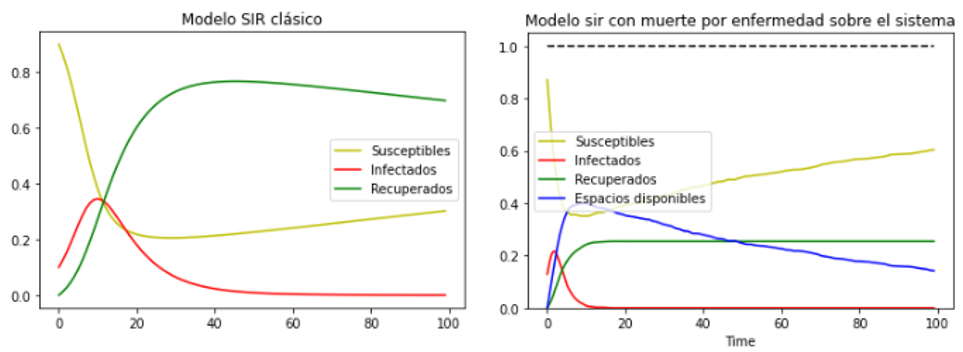
\includegraphics[width=0.9\textwidth]{Imagenes/solucionesMuertePorEnfermedad.PNG}
    \caption{Evolución de la enfermedad en 100 bimestres (modelo clásico y regla $\theta_{SIR,6}^t(x)$)}
\end{figure}
Se evidencia un pico para la enfermedad en las primeras iteraciones, esto se debe principalmente a la alta tasa de contagio. Sin embargo, la alta tasa de muerte causada por la enfermedad hace que esta población desaparezca rápidamente como observa en ambos modelos.

Una diferencia significativa se puede apreciar en la cantidad promedio de contagios. En el caso del modelo en autómatas celulares podemos afirmar que el número de contagios pudo no haber crecido en gran medida por algo como lo que se observa en la figura (\ref{fig:muertePorEnfermedad10Veces}), en donde las limitadas relaciones de las células hacen que los individuos infectados tiendan a aislarse.
\end{example}

En el siguiente capítulo analizaremos diferentes tipos de vecindades y expondremos sus diferencias e implicaciones dentro del estudio epidemiológico, esto con el fin de apreciar comportamientos como el mencionado en el ejemplo \ref{ex:muertePorEnfermedadClásicovsModeloEnAC}.

\include{Contenidos/C4-ComparaciónConModelosClasicos}
\chapter{Conclusiones}

Al realizar este trabajo, se comprendió la naturaleza dinámica de los modelos basados en compartimientos que describen el comportamiento de los estados que caracterizan un fenómeno propagativo en un conjunto establecido. Así mismo, las propiedades de los autómatas celulares que permiten describir comportamientos espaciales a gran escala, a partir de conceptos básicos de topología como lo son los sistemas fundamentales de vecindades, las relaciones de orden parcial que definen los conjuntos $\mathcal{V}(x)$ dada una topología cualquiera, entre otros. El entendimiento de estos conceptos permitió establecer una relación entre las interacciones entre los individuos de algún sistema finito con los sistemas fundamentales de vecindades y esto a su vez nos planteó una visión clara de la incidencia de la naturaleza de las interacciones y las frecuencias con las que ocurren,
en la evolución de una enfermedad.

Las conclusiones que se pueden enunciar de este trabajo son:
\begin{itemize}
    \item Haciendo uso de las propiedades de los autómatas celulares para describir comportamientos espaciales y de los sistemas fundamentales de vecindades es posible modelar las relaciones sociales de un conjunto de individuos determinado.
    \item Las condiciones iniciales sobre la manera en la que interactúan las células no impacta a los puntos de equilibrio de las curvas que describen el comportamiento de la enfermedad.
    \item Se evidencia que limitar y/o reducir la intensidad de las interacciones sociales es una medida efectiva para disminuir los casos de individuos infectados.
    \item Se comprobó que es posible alcanzar una inmunidad de rebaño si se reducen significativamente las interacciones entre individuos.
    \item Las reglas y algoritmos propuestos permiten visualizar de manera clara e intuitiva a la manera en la que una enfermedad evoluciona dentro de una población, manteniendo un comportamiento que puede ser descrito en cierta medida por los modelos compartimentales clásicos.
    \item Si bien las reglas planteadas permiten analizar características que no eran posibles con los modelos clásicos, se evidencia una limitación en cuanto a que se asume una capacidad máxima de individuos en el sistema.
    \item La metodología empleada para el diseño e implementación de las reglas de evolución descritas en este trabajo, brindan un camino claro para la definición de reglas que modelen el comportamiento de modelos epidemiológicos más generales.
\end{itemize}
\include{Contenidos/C6-Apéndices}

\addcontentsline{toc}{chapter}{\numberline{}Bibliografía}
%   \nocite{*}
  \bibliography{BibliMSc}
  \bibliographystyle{abbrv}
\end{document}